
\documentclass{beamer}

\usepackage{color}
\usepackage{amsthm}
\usepackage{hyperref}
\usepackage{beamerthemesplit}
\usetheme{Madrid}
\usecolortheme{wolverine}
%\setbeamertemplate{pgfdeclareverticalshading}
%{beamer@headfade}{\paperwidth}
%{
%  color(0cm)=orange;
%  color(1.25cm)=orange;
%}
\setbeamertemplate{footline}
       {
%%      \leavevmode%
%%      \hbox{%
%%      \begin{beamercolorbox}[wd=.333333\paperwidth,ht=2.25ex,dp=1ex,center]{author in head/foot}%
%%        \usebeamerfont{author in head/foot}\insertshortauthor~~(\insertshortinstitute)
%%      \end{beamercolorbox}%
%%      \begin{beamercolorbox}[wd=.333333\paperwidth,ht=2.25ex,dp=1ex,center]{title in head/foot}%
%%        \usebeamerfont{title in head/foot}\insertshorttitle
%%      \end{beamercolorbox}%
%%      \begin{beamercolorbox}[wd=.333333\paperwidth,ht=2.25ex,dp=1ex,right]{date in head/foot}%
%%        \usebeamerfont{date in head/foot}\insertshortdate{}\hspace*{2em}

%%    %#turning the next line into a comment, erases the frame numbers
%%        %\insertframenumber{} / \inserttotalframenumber\hspace*{2ex}

%%      \end{beamercolorbox}}%
%%      \vskip0pt%
   }
\setbeamertemplate{navigation symbols}{}



%\documentclass{beamer}

%\documentclass{article}
%\usepackage[language]{babel}
%\usepackage[top=1in, left=1in, right=1in, bottom=1in]{geometry}
\usepackage{amsmath,amssymb,amsthm,graphicx}
\usepackage{subfigure}
\usepackage{wrapfig}
\usepackage{multirow}
\usepackage{listings}
\usepackage{color}
\usepackage{bm}
\usepackage{hyperref}
%\usetheme{default}
%\usetheme{Gerrish}
\usepackage[mathcal]{euscript}   % for script letters

\setbeamertemplate{navigation symbols}{}
\setbeamertemplate{outlinem}{}


%\setbeamertemplate{frametitle}{}
%\setbeamertemplate{frametitle}{}

%\addtoheadtemplate{\pgfuseshading{beamer@headfade}\vskip-1.25cm}{sadsdf}

\newcommand{\z}{\textbf{z}}
\newcommand{\W}{\textbf{W}}
\newcommand{\mv}{\tilde{m}} 
\newcommand{\vv}[0]{\tilde{V}}
\newcommand{\w}{\textbf{w}}
\newcommand{\vphi}{\phi}
\newcommand{\bv}{\tilde{\beta}}
\newcommand{\bb}{\beta}
\newcommand{\lv}{\tilde{l}}
\newcommand{\vlv}{\sigma^2_{l}}
\newcommand{\vd}{\sigma^2_{d}}
\newcommand{\vbv}{\sigma^2}
\newcommand{\stdnorm}[1]{\mathcal{N}\left(#1\right)}


\newcommand{\tr}[0]{\mbox{Tr}}
% \newcommand{\expect}[1]{\mathbb{E}\left[#1\right]}
\newcommand{\expectq}[1]{\mathbb{E}_q\left[#1\right]}
\newcommand{\expectqnoarg}[0]{\mathbb{E}_q}
\newcommand{\defn}[0]{:=}
\newcommand{\partl}[2]{\frac{\partial #1}{\partial #2}}

\definecolor{yellow}{rgb}{0.9,0.9,0.4}

\title{A Language-based Approach to Measuring Scholarly Impact}
 \subtitle{} \date{22 June 2010} \author{Sean Gerrish and David Blei \newline Princeton University}

\begin{document}

\section*{Outline}

\frame{\titlepage}

\section{Introduction}

\frame {
%  When did people become excited about mad cow disease?
%  \begin{figure}
%    \includegraphics[width=0.4\textwidth]{../figures/400px-CH_cow_2.jpg}
%    \newline \tiny Image author Daniel Schwen;
%    \newline available 13 April 2010 at \href{http://commons.wikimedia.org/wiki/File:CH_cow_2.jpg}{Wikipedia}
%    \normalsize
%  \end{figure}
\frametitle{Identifying influential documents}


\begin{itemize}
\item In large collections of text documents, which ones are important?

\begin{center}

\includegraphics[width=0.4\textwidth]{figs/documents.jpg} \newline
\tiny Image source: \url{http://jenslapinski.files.wordpress.com/2008/06/documents.jpg}
\end{center}
\normalsize

\item We have developed a statistical model to measure the influence of text documents.
  
\item Based only on the language of the documents, this measure is
  significantly correlated to citation counts.

\end{itemize}

}

\subsection{The problem}

\frame {
 \frametitle{Identifying influential documents}

%\begin{center}
%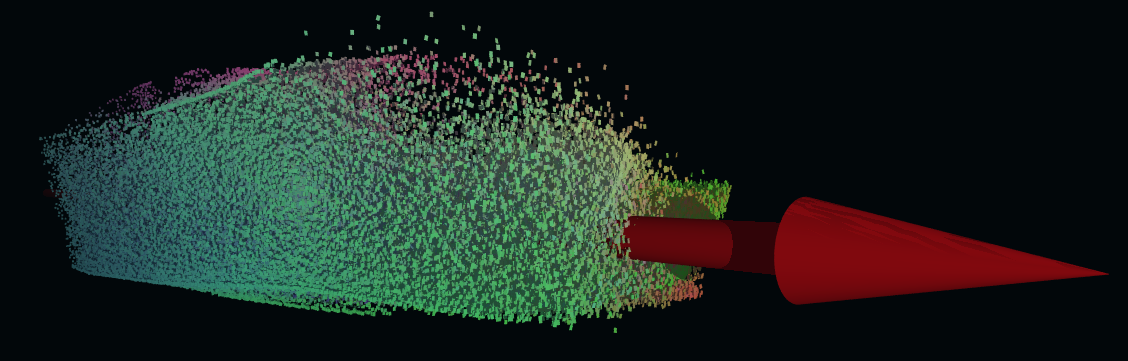
\includegraphics[width=0.9\textwidth]{../figures/docs_basic.png} \newline
%\end{center}
 \begin{itemize}
 \item Goal: Develop a measure of influence based only on language.
 \item There are many specific application areas.
   \begin{itemize}
   \item News articles
   \item Legal opinions
   \item Scientific impact
     %   \item Transcriptions of radio content and orations
     \\
   \end{itemize}
 \item  Entire fields of study rely on work like this.
   \begin{itemize}
   \item History
   \item Academic research
   \item Much of Bibliometrics
   \end{itemize}
 \end{itemize}
}

\frame {
  \frametitle{Common approach: citations}

  \begin{figure}
    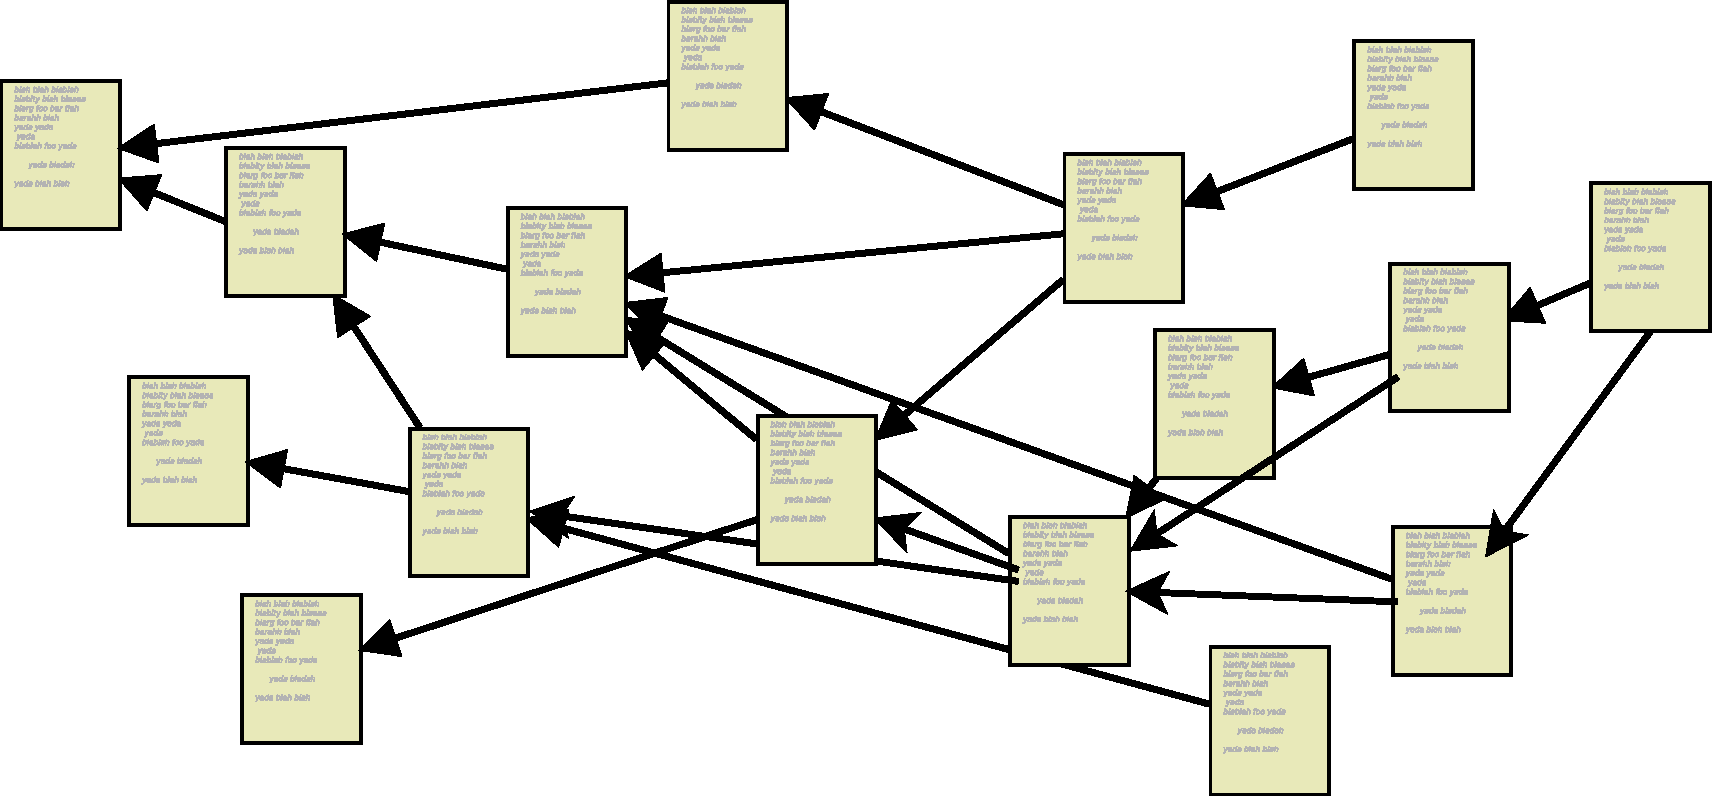
\includegraphics[width=0.75\textwidth]{figs/citation_network.pdf}
  \end{figure}
  \begin{itemize}
    \item Traditionally, citations are used to identify influential documents.
    \item E.g.: \emph{A novel progressive spongiform encephalopathy in
      cattle}, \cite{wells:1987}
      (Cited by 709)
\vspace{2in}
  \end{itemize}
}

\frame {
  \frametitle{Common approach: citations}
  \begin{figure}
    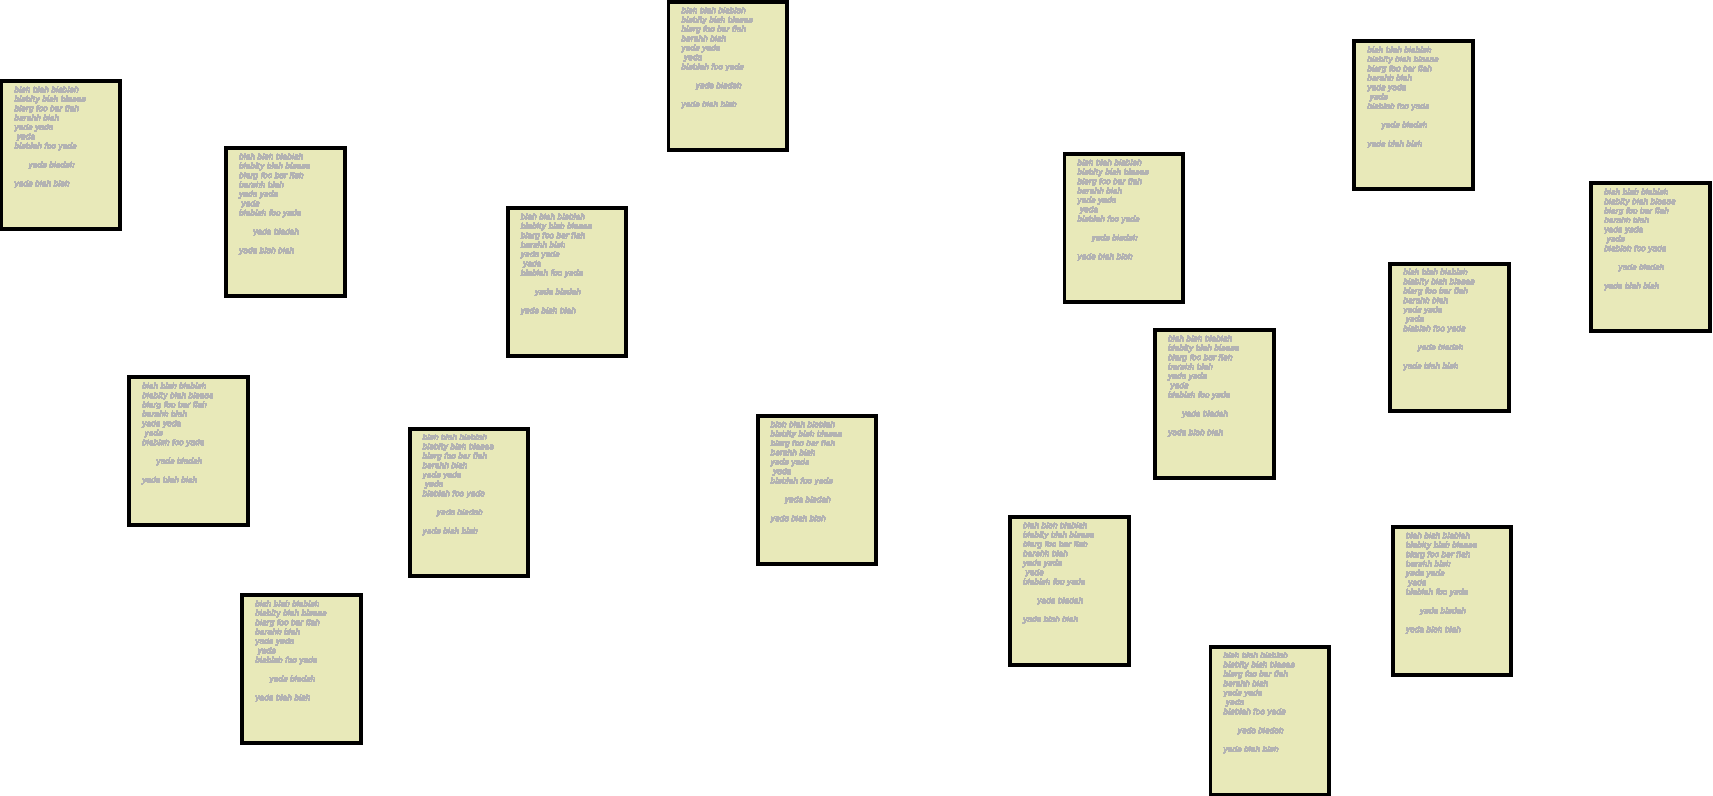
\includegraphics[width=0.75\textwidth]{figs/no_citation_network.pdf}
  \end{figure}
  \begin{itemize}
    \item Citations are limited
      \begin{itemize}
      \item May not exist
      \item Hard to get
      \item Describe only one kind of influence
      \end{itemize}
    \item A language-based approach enables us to measure the influence of
      new kinds of documents
      \begin{itemize}
      \item News articles
      \item Historic manuscripts
      \end{itemize}
  \end{itemize}
}


%% \frame {
%%  \frametitle{Predicting influence in the absence of citations}
%%   \begin{figure}
%%     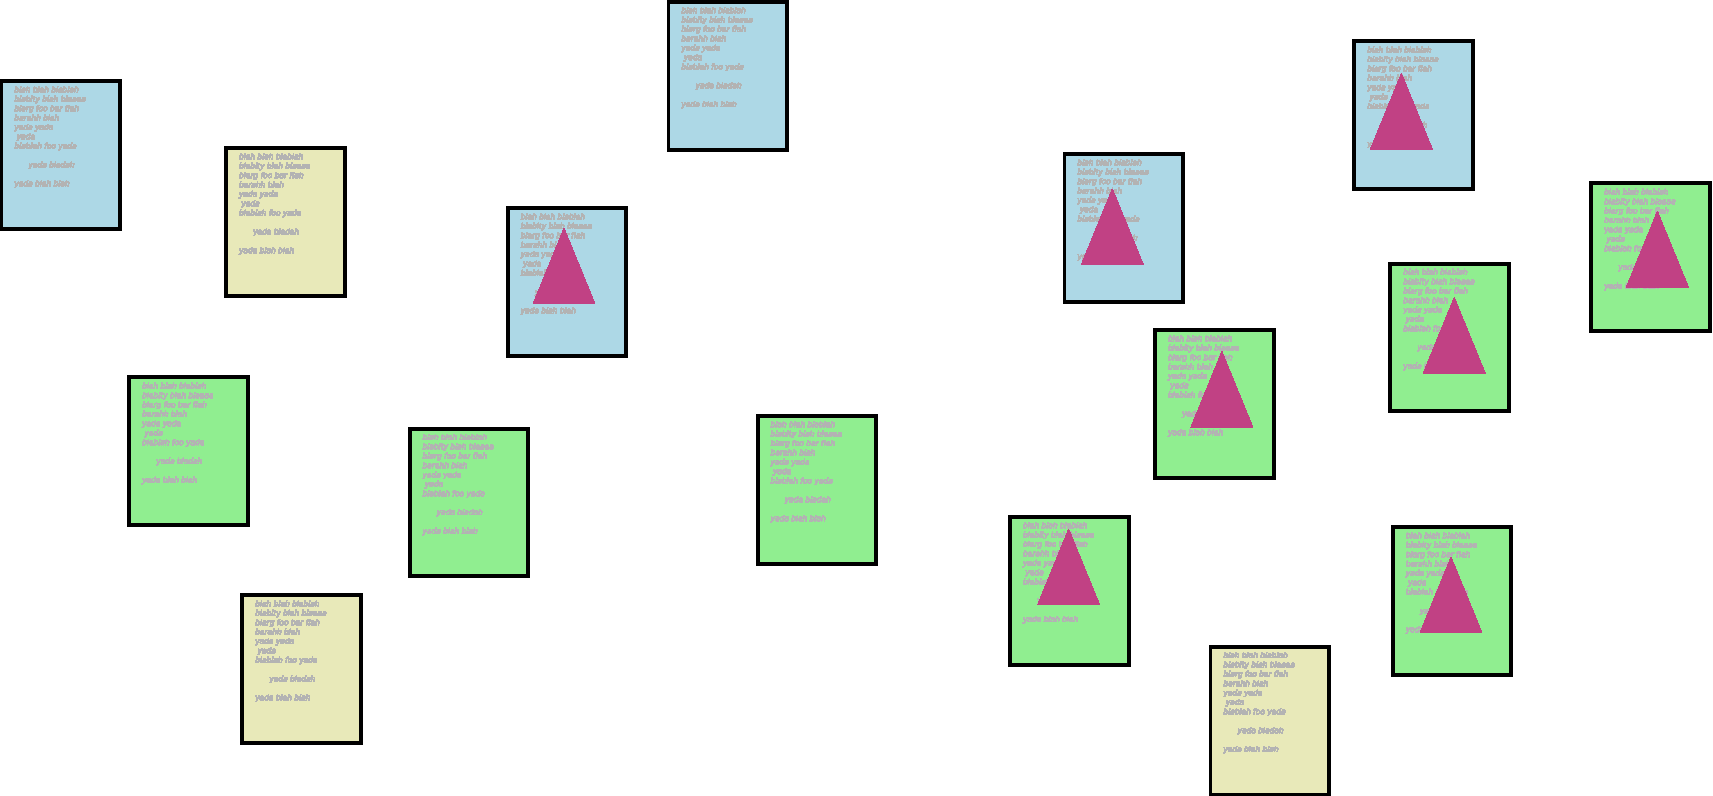
\includegraphics[width=0.8\textwidth]{../figures/topic_network.pdf}
%%   \end{figure}

%%   \begin{itemize}
%%     \item \label{def} Our \emph{intuition} is that influential
%%       documents change the language of their fields.
%%     \item Our \emph{goal} is to model the influence of documents
%%       without additional information.
%%   \end{itemize}
%%   Note that we assume documents influence their own subfields, not the
%% entire corpus.
%% \vspace{1in}
%% }

\frame {
  \frametitle{Methodology}
  \vspace{-.05in}
  \begin{centering}
    \begin{figure}
    \hspace{0in} 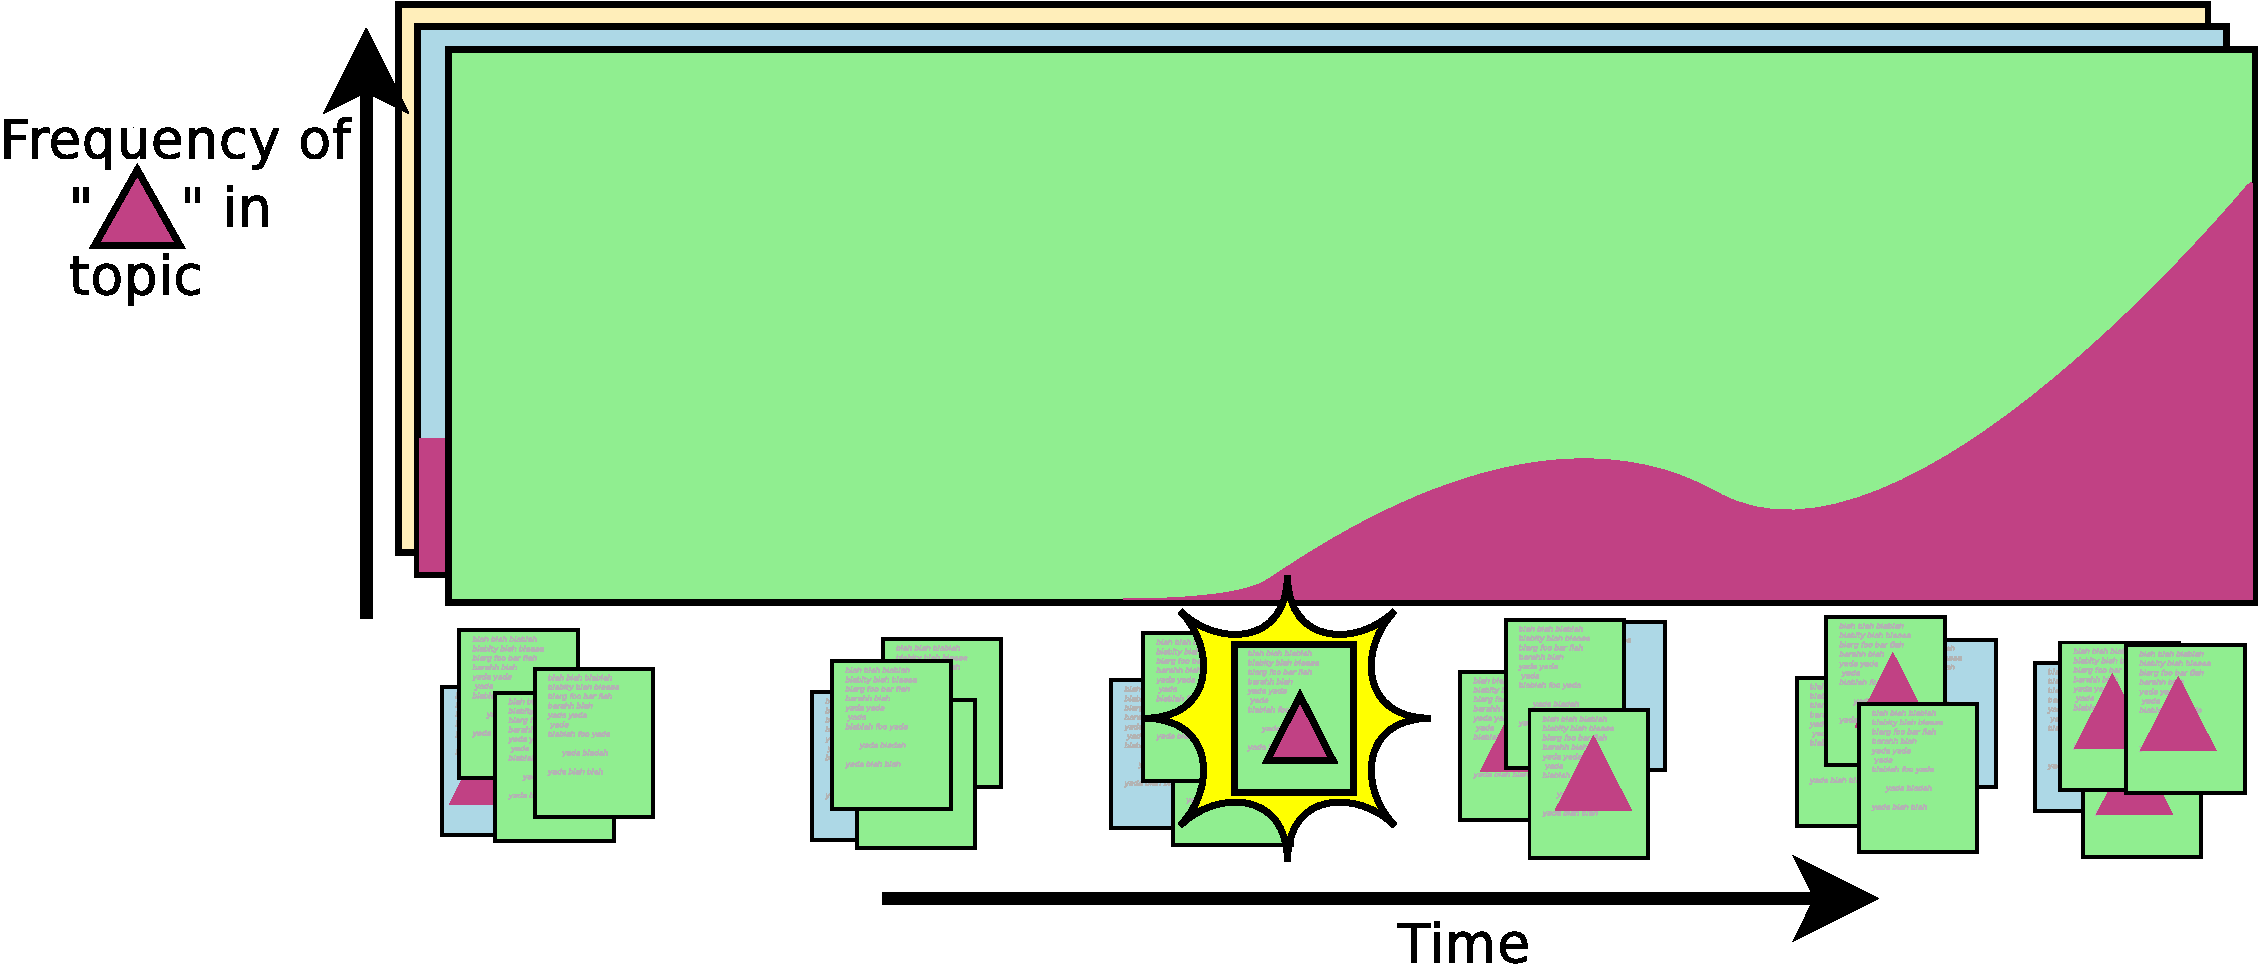
\includegraphics[width=0.8\textwidth]{figs/influence_intuition.pdf} \newline
%    \begin{figure}
%      \includegraphics[width=0.4\textwidth]{../figures/docinf_gm.pdf}
%    \end{figure}
    \end{figure}
  \end{centering}
  \vspace{-.25in}
  \small
  \begin{itemize}
  \item We develop a probabilistic model to captures the influence of documents.
    %    \item Build assumptions from \emph{topic models} into this model
  \item The intuition: influential documents use language that becomes more popular in later years.
  \item With posterior inference, we retrospectively see which documents have been influential on the corpus.
%  \item Related to \cite{leskovec:2009} and [Shaparenko et al., 2007], with a focus on topics.  
  \end{itemize}
  \normalsize
}

\section{Topic Models and LDA}

\frame {
  \frametitle{Changing topics}
  \begin{itemize}
    \item Topic models decompose a corpus into a set of topics, i.e. distributions over terms.
    \item The Dynamic Topic Model allows topics to change over time \cite{blei:2006}.

      \begin{figure}
        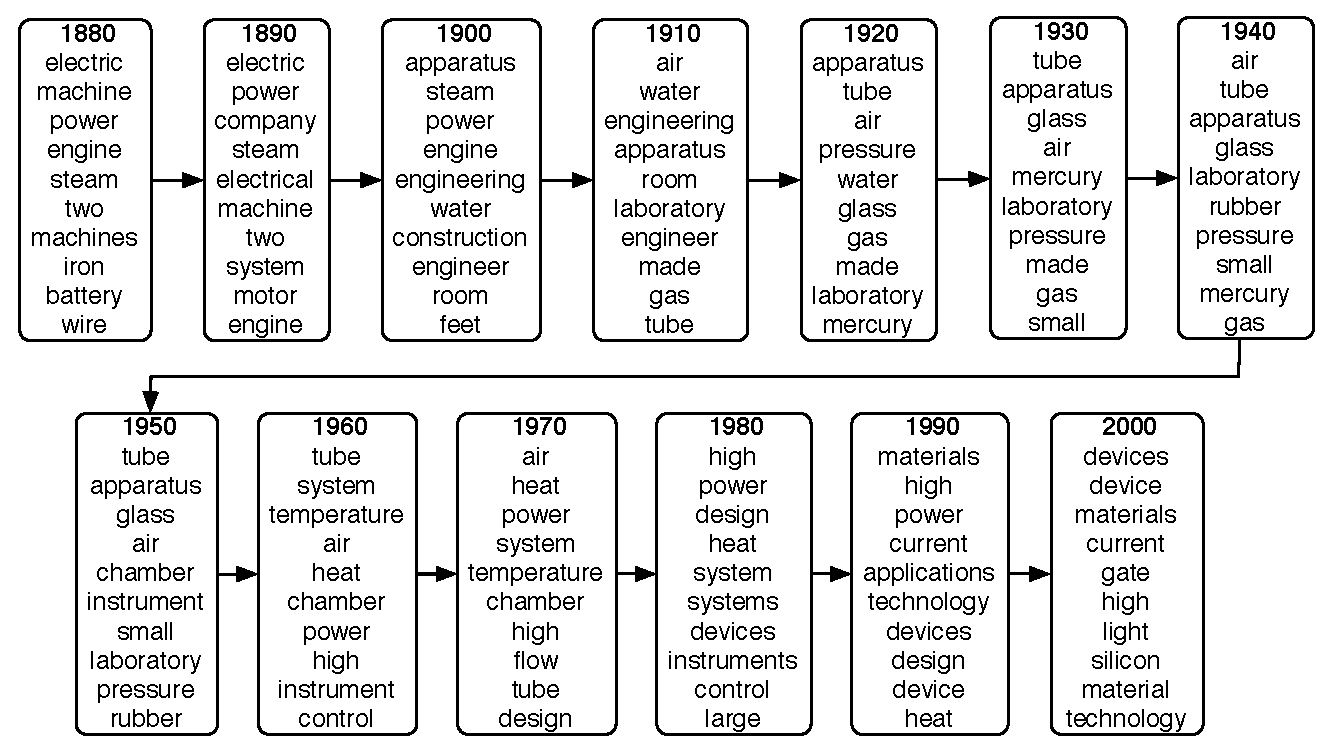
\includegraphics[width=0.8\textwidth]{figs/devices-topic-34.pdf}
      \end{figure}
  \end{itemize}
}

%% \frame {
%%   \frametitle{Topic models}
%%   \begin{itemize}
%%     \item Topic models help to identify latent themes in document collections (like text, images)

%%       \begin{figure}
%% 	\vspace{-5pt}
%% 	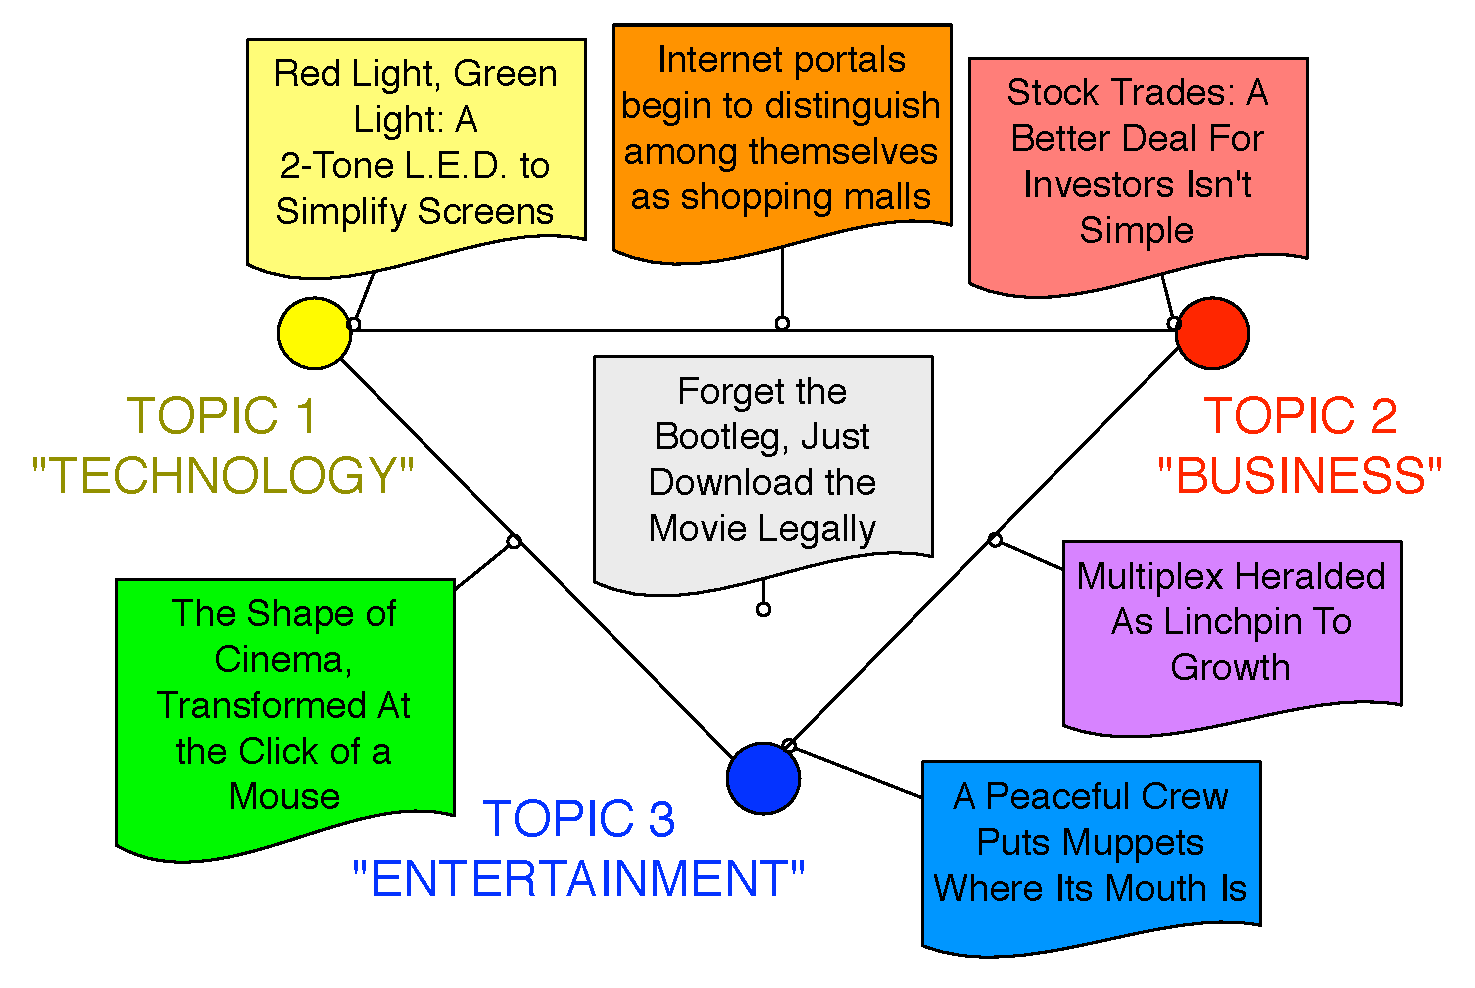
\includegraphics[width=0.7\textwidth]{../figures/nyt_documents.pdf}
%% 	\newline \tiny Image source \cite{changrtl:2009} \normalsize
%%       \end{figure}

%%       We use Latent Dirichlet Allocation (LDA) \cite{blei:2003}
%%   \end{itemize}
%% }

%% \frame{

%% \frametitle{Topics}

%% We use posterior inference to discover these topics automatically.

%% An LDA topic is formally a probability
%% distribution over words.
%% \newline
%% Some topics from JSTOR: \newline
%%   \begin{itemize}
%%     \item agricultural, land, farm, environmental, water \newline
%%     \item infection, patients, virus, cancer, mice \newline
%%     \item health, nursing, nurses, hospital, medical \newline
%%     \item theorem, lemma, proof, finite, algebra \newline
%%   \end{itemize}
%% }

%% \frame { \frametitle{Latent Dirichlet Allocation} LDA assumes
%%   documents are generated from a generative model.
%%   \newline
%%   Posterior influence is like ``filling in'' the hidden variables.
%%   \newline
%%   Given a set of topics $\beta$, draw a document as follows:
%%   \begin{columns}
%%     \begin{column}[left]{0.66\linewidth}
%%       \begin{itemize}
%% 	\item Choose topic mixture $\theta \sim \mbox{Dir}(\bm \alpha)$.
%% 	  \newline For each term:
%% 	\begin{itemize}
%% 	  \item Choose a topic indicator $z_n \sim \mbox{Multinomial}(\theta)$.
%% 	  \item Choose a word $w_n \sim p(w_n | z_n, \beta)$.
%% 	\end{itemize}
%%       \end{itemize}
%%       \end{column}
%%     \begin{column}[center]{0.34\linewidth}
%%       \begin{figure}
%%       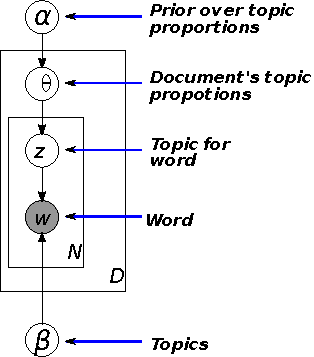
\includegraphics[width=1\textwidth]{../figures/lda.pdf}
%%       \end{figure}
%%     \end{column}
%%   \end{columns}
%% }

\section{Model}



%% \frame {
%%   \frametitle{The Dynamic Topic Model}

%%   Assumes topics drift in a Markov chain:\newline
%%   $\beta_t \sim \mathcal{N}(\beta_{t-1}, \sigma^2)$  \newline
%%   $D_t \sim$ LDA($\alpha_t, \beta_t$) \newline

%%   \begin{columns}
%%     \begin{column}[left]{0.5\linewidth}
%%       \begin{figure}
%% 	\vspace{-8pt}
%% 	\hspace{105pt}
%% 	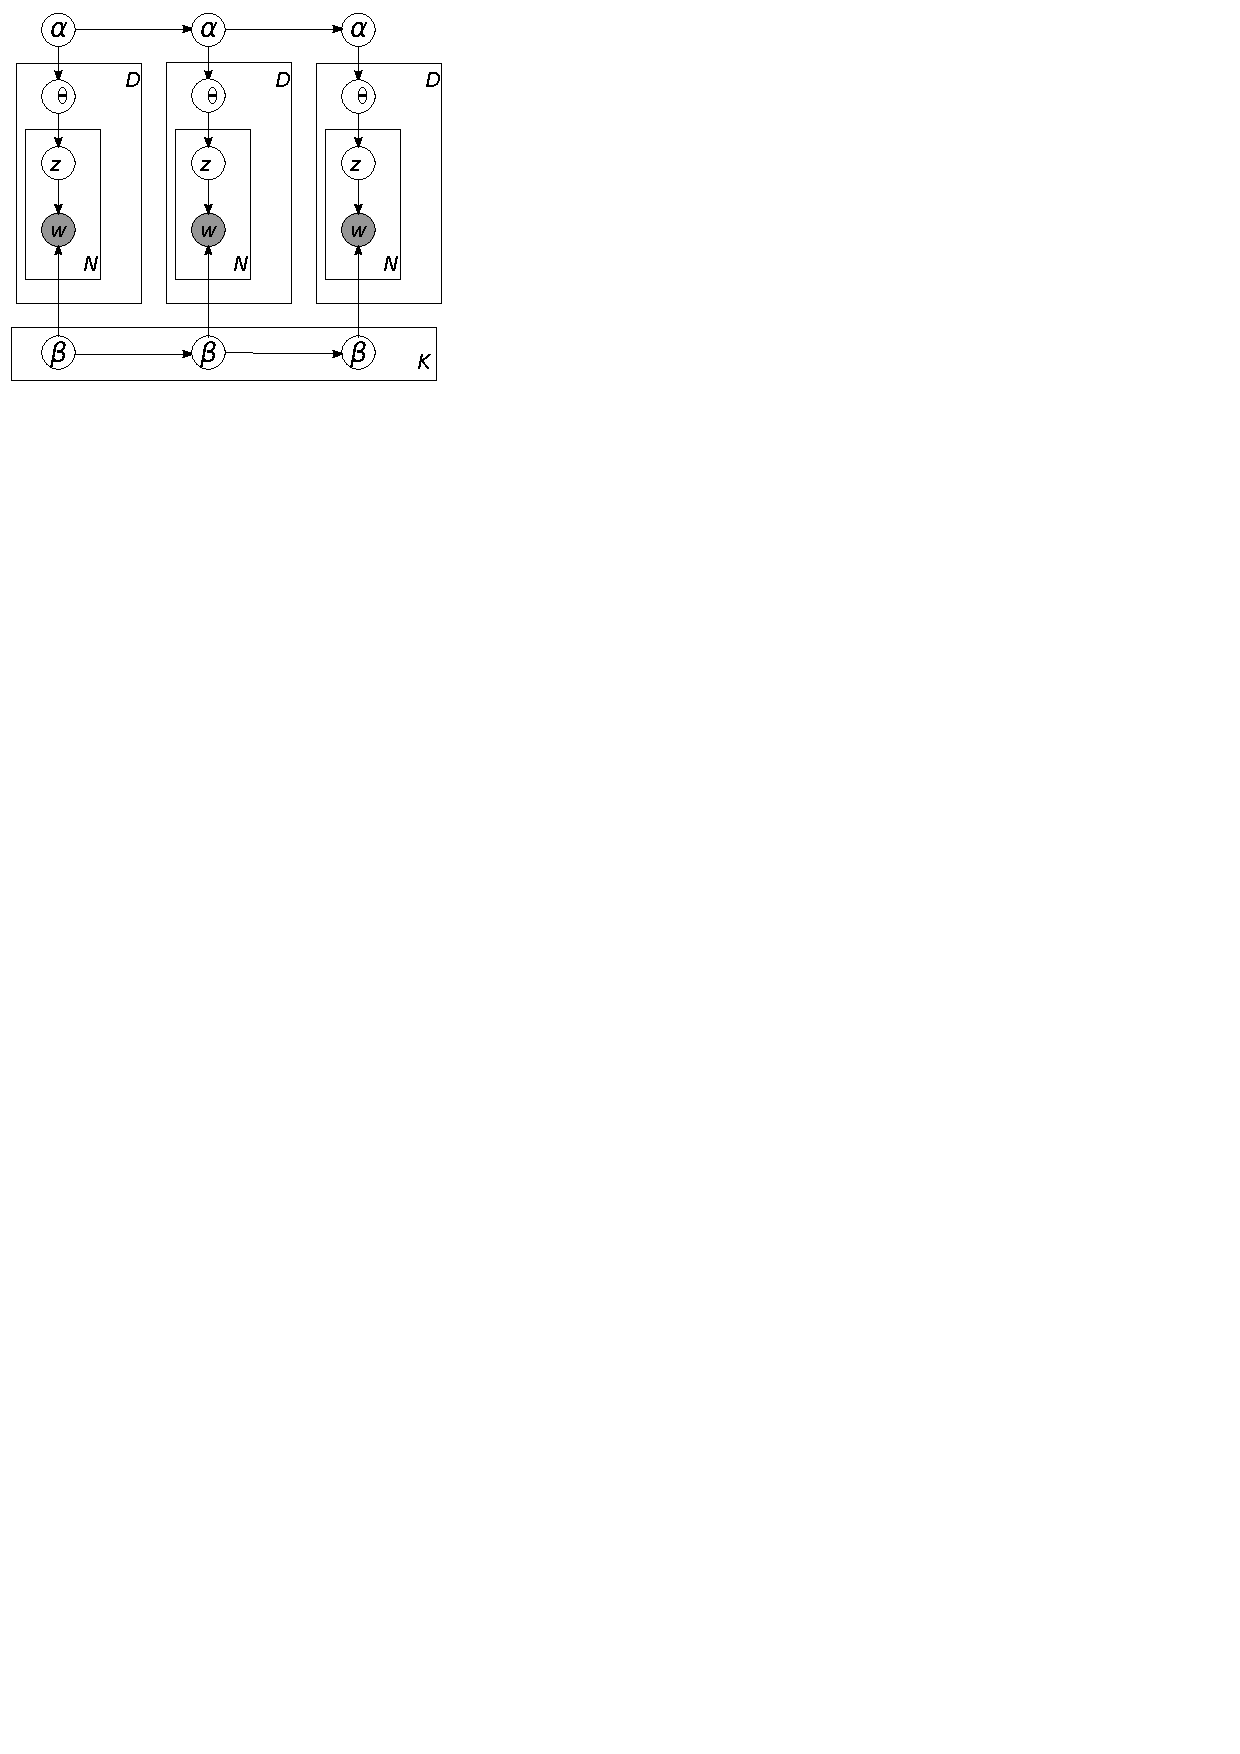
\includegraphics[width=3.0\linewidth]{../figures/dtm.pdf}
%%       \end{figure}
%%     \end{column}
%%     \begin{column}[left]{0.5\linewidth}
%%       \vspace{-500pt}
%%       For time $t = 1, \ldots, T$:
%%       \begin{itemize}
%%       \item For topic $k = 1, \ldots, K$: \label{gen:beta} \\
%% 	Draw natural parameters $\beta_{t,k} | \beta_{t-1,k}, \sigma^2 I$
%%       \item For each document $d_t$:
%%         \begin{itemize}
%%    	\item Generate document $d_t$ using traditional LDA with parameters
%% 	  $\alpha_t$ and $\beta_{t}$.
%%         \end{itemize}
%%       \end{itemize}

%%     \end{column}
%%   \end{columns}
%% }

\frame {
  \frametitle{The Dynamic Topic Model}
  \begin{itemize}
  \item Topics drift in a Markov chain:\newline
     $\beta_t \sim \mathcal{N}(\beta_{t-1}, \sigma^2)$ \newline
  \item Documents are generated from Latent Dirichlet Allocation \newline
     $D_t \sim$ LDA($\alpha_t, \beta_t$) \newline

   \end{itemize}
   % Assumes each document has a weight which affects topic drift...\newline
%     $l_{d,k} \sim \mathcal{N}(0, \sigma_l^2)$ \newline
\vspace{-0.43in}
  \begin{figure}
    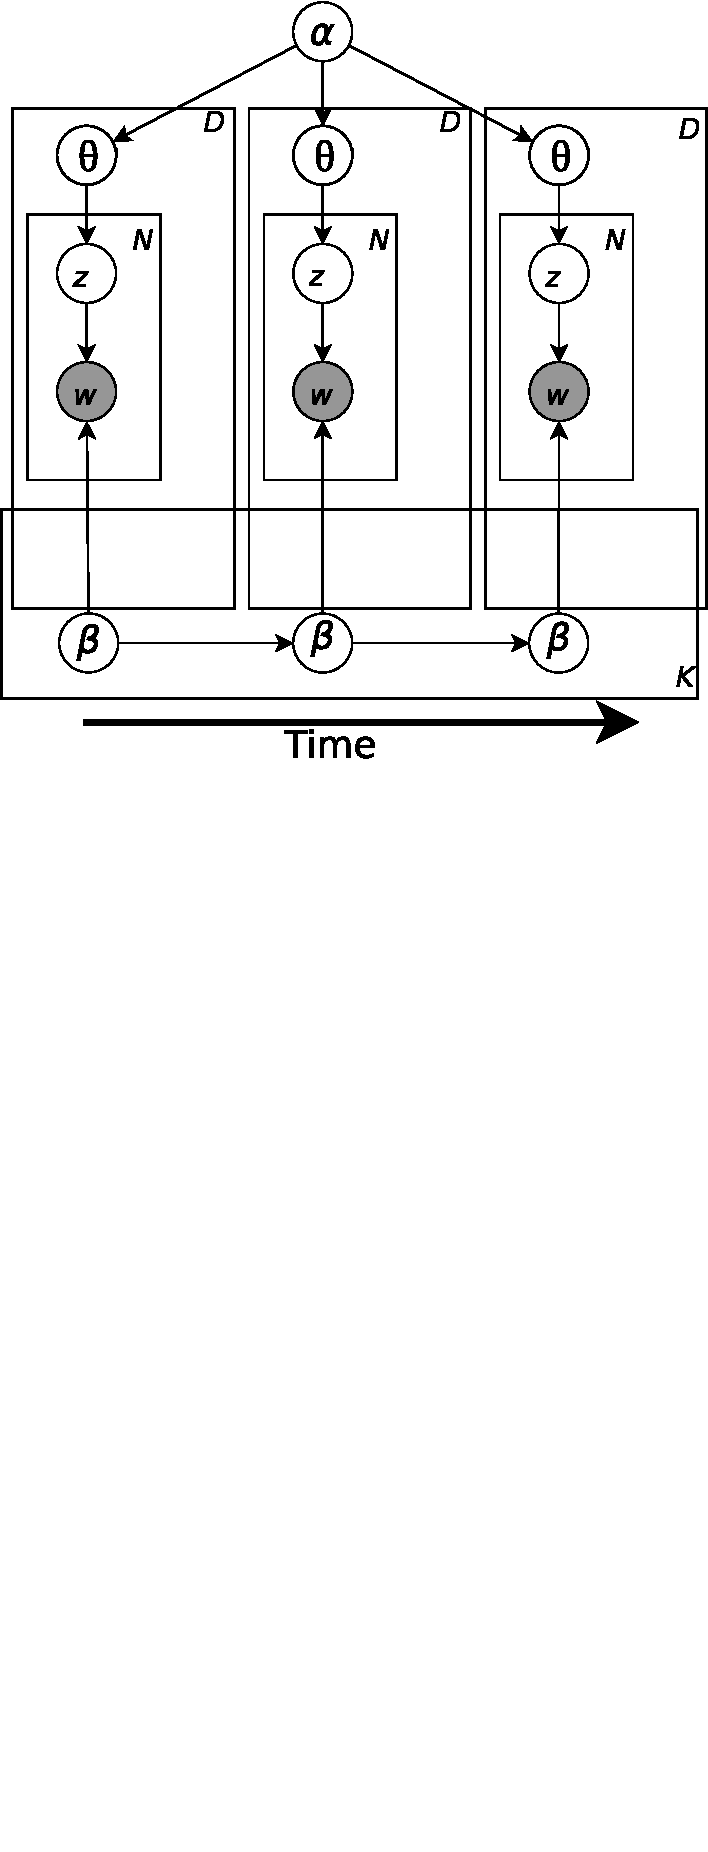
\includegraphics[width=0.44\linewidth]{figs/dtm_gm.pdf}
  \end{figure}
}

\frame {
  \frametitle{The Document Influence Model}
  \begin{itemize}
  \item Topics drift in a Markov chain:\newline
     $\beta_t \sim \mathcal{N}(\beta_{t-1} \textcolor{blue}{ + \mbox{Infl}(...)}, \sigma^2)$ \newline
  \item Documents are generated from Latent Dirichlet Allocation \newline
     $D_t \sim$ LDA($\alpha_t, \beta_t$) \newline

   \end{itemize}
   % Assumes each document has a weight which affects topic drift...\newline
%     $l_{d,k} \sim \mathcal{N}(0, \sigma_l^2)$ \newline
\vspace{-0.43in}
  \begin{figure}
    \includegraphics[width=0.44\linewidth]{figs/docinf_gm.pdf}
  \end{figure}
}

%% \frame {
%%   \frametitle{The Document Influence Model}
%%   ... with documents having potential influence in the distant future. \newline
%%   $l_{d,k} \sim \mathcal{N}(0, \sigma_l^2)$ \newline
%%   $\beta_t \sim \mathcal{N}(\beta_{t-1} + \mbox{Inf}(l_{s<t}, z_{s<t}, w_{s<t}), \sigma^2)$ \newline
%%   $D_t \sim$ LDA($\alpha_t, \beta_t$)
%%   \begin{figure}
%%     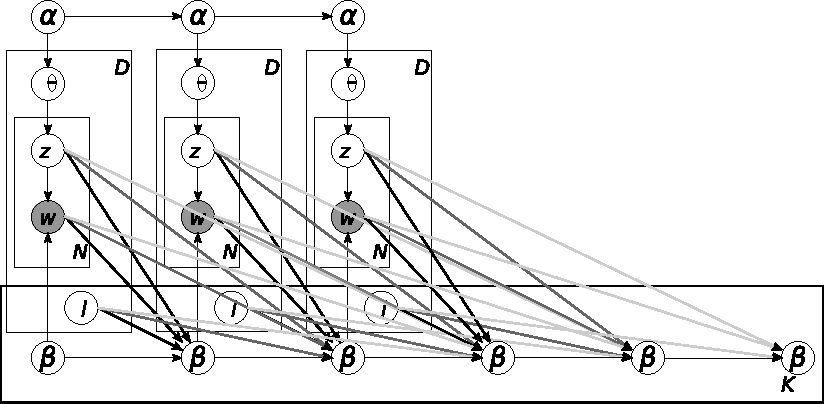
\includegraphics[width=1.0\linewidth]{../figures/docinf_gm_all_arrows.pdf}
%%   \end{figure}
%% }

\frame{ \frametitle{The DIM influence function}
  Markov step: $\beta_{t,k} \sim \mathcal{N}(\beta_{t-1,k} + \textcolor{blue}{Infl(t,k)}, \sigma^2 I)$,
  \newline
  We developed the model to have certain characteristics:
  \begin{itemize}
    \item More recent documents have greater influence.
    \item A document only influences relevant topics.
  \end{itemize}
  \begin{figure}
    \includegraphics[width=0.9\linewidth]{figs/influence_function_new.pdf}
  \end{figure}
}

%% \frame{
%%   \frametitle{The DIM influence function}
%%   Markov step: $\beta_{t,k} \sim \mathcal{N}(\beta_{t-1,k} + \textcolor{blue}{Infl(t,k)}, \sigma^2 I)$, \newline
%%   $\textcolor{blue}{Infl(s,k)} := $\textcolor{black}{$\exp(-\beta_{s-1,k})$}$ \circ \sum_{i=0}^{s-1} \textcolor{black}{r(s - 1 - i)}
%%     (\textcolor{black}{[\z_{i}]_k} \circ \W_{i}) l_{i,k}$,
%%   \begin{itemize}
%%   \item $\textcolor{black}{r(j)}$ is the fraction of a document's influence after $j$
%%     years (called the influence envelope)
%%   \item $\textcolor{black}{[z]_k}$ is the indicator describing whether term $z$ is in
%%     topic $k$
%%   \item \textcolor{black}{$\exp(-\beta_{s-1,k})$} means we add inches to inches and not to log(inches)
%%   \end{itemize}
%%   \begin{figure}
%%     \includegraphics[width=0.9\linewidth]{../figures/influence_function_new.pdf}
%%  \end{figure}
%% }

\frame {
  \frametitle{How do we find the model parameters?}
  \begin{itemize}
    \item We observe only the words $\bm w$.
    \item We want to find the posterior $p(I, \theta, z, \beta | \bm w)$.
    \item We use variational methods \cite{jordan:1999}.
  \end{itemize}
  \begin{centering}
    \begin{figure}
      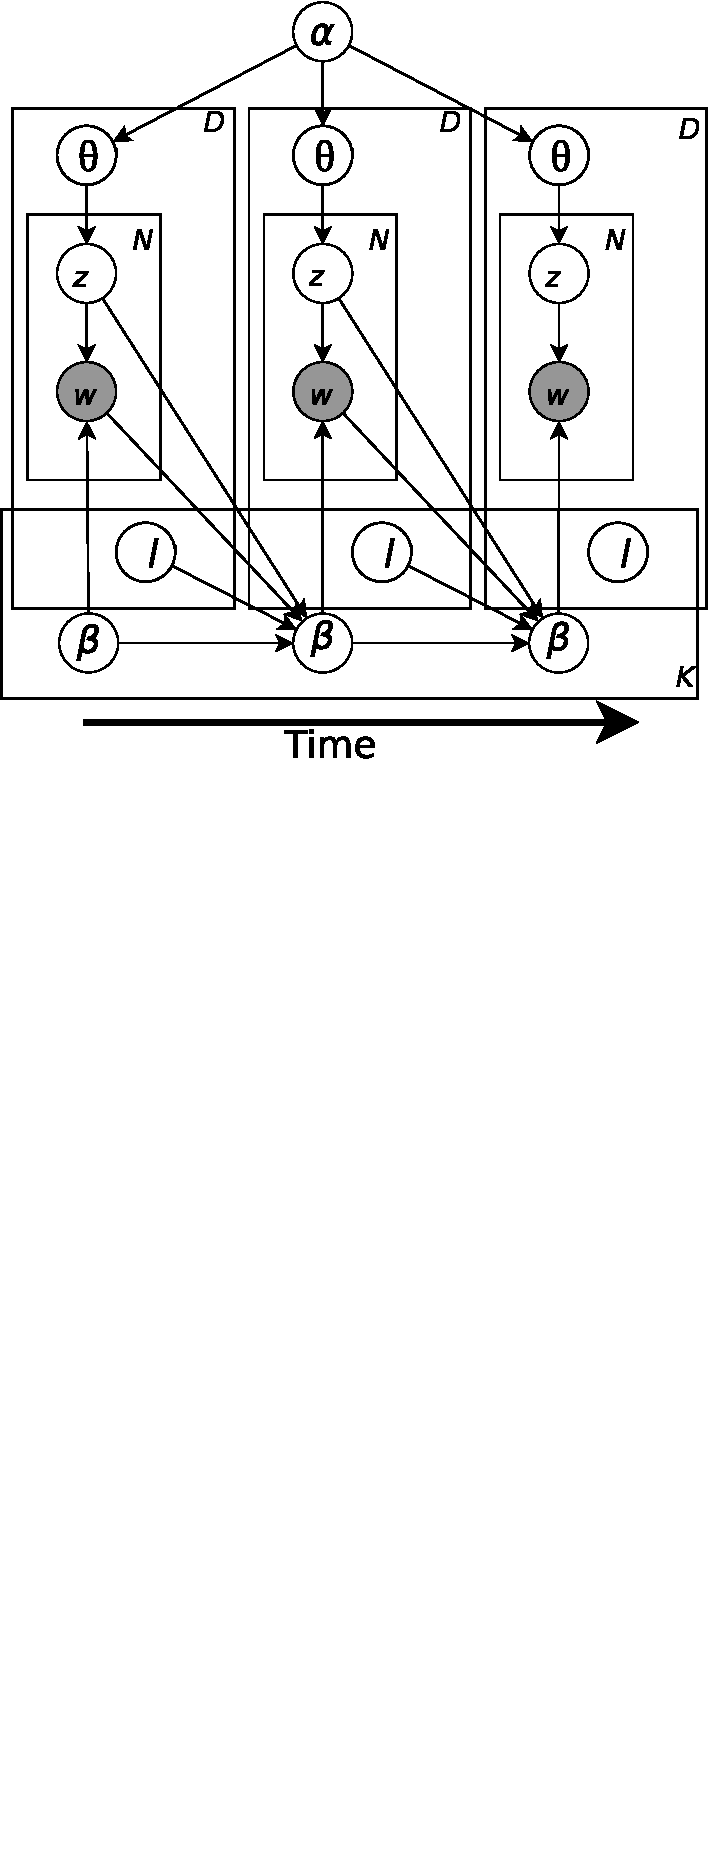
\includegraphics[width=0.5\textwidth]{figs/docinf_gm_bw.pdf}
    \end{figure}
  \end{centering}
}

%% \frame {
%%   \frametitle{We use variational inference}
%%   \begin{itemize}
%%     \item Variational inference approximates the posterior density $p(x | \bm w)$ with some distribution $q(x)$.
%%     \item $q(x)$ comes from a simplified family of distributions. \cite{jordan:1999}
%%     \item We find $q(x)$ by minimizing $KL(q || p(x | \bm w))$.
%%   \end{itemize}
%%   \begin{centering}
%%     \begin{figure}
%%       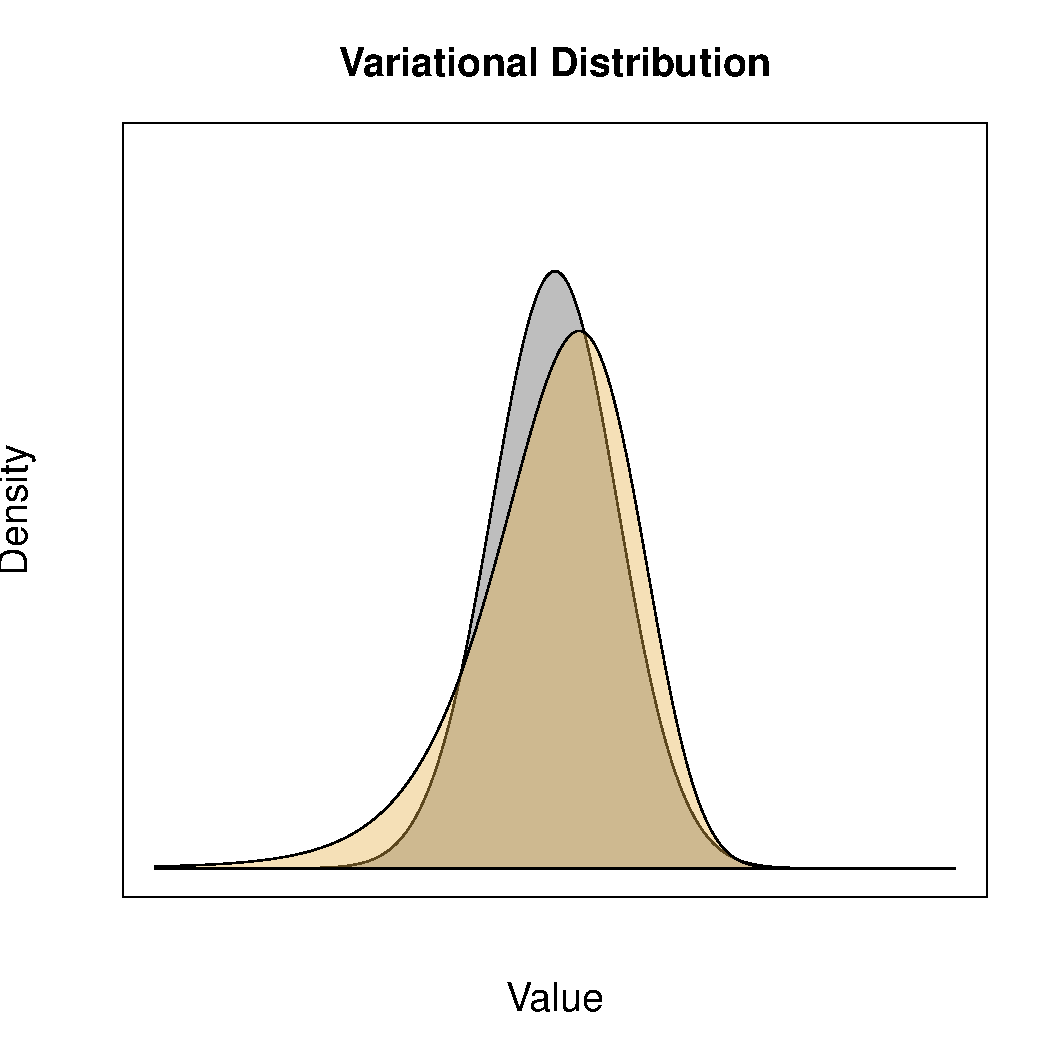
\includegraphics[width=0.5\textwidth]{../figures/variational_distribution.jpg} \\
%%     \end{figure}
%%   \end{centering}
%% }

\frame{
  \frametitle{Experiments}
  \begin{itemize}
  \item We analyzed three corpora with the DIM.
    \begin{itemize}
    \item The \emph{ACL Anthology}: 7561 documents
    \item \emph{Nature}: 34454 documents
    \item \emph{PNAS}: 11855 documents
    \end{itemize}
  \item This provides estimates of the influence of each article.
  \item We computed the Spearman rank correlation with citations.
    \begin{itemize}
    \item ACL Anthology Network \cite{Radev:2009}
    \item Google Scholar (PNAS and Nature)
    \end{itemize}
  \end{itemize}
    
}

\frame {
  \frametitle{Topics in ACL and PNAS}
% \emph{Using Restriction To Extend Parsing Algorithms For Complex-Feature-Based Formalisms}
  \begin{figure}
    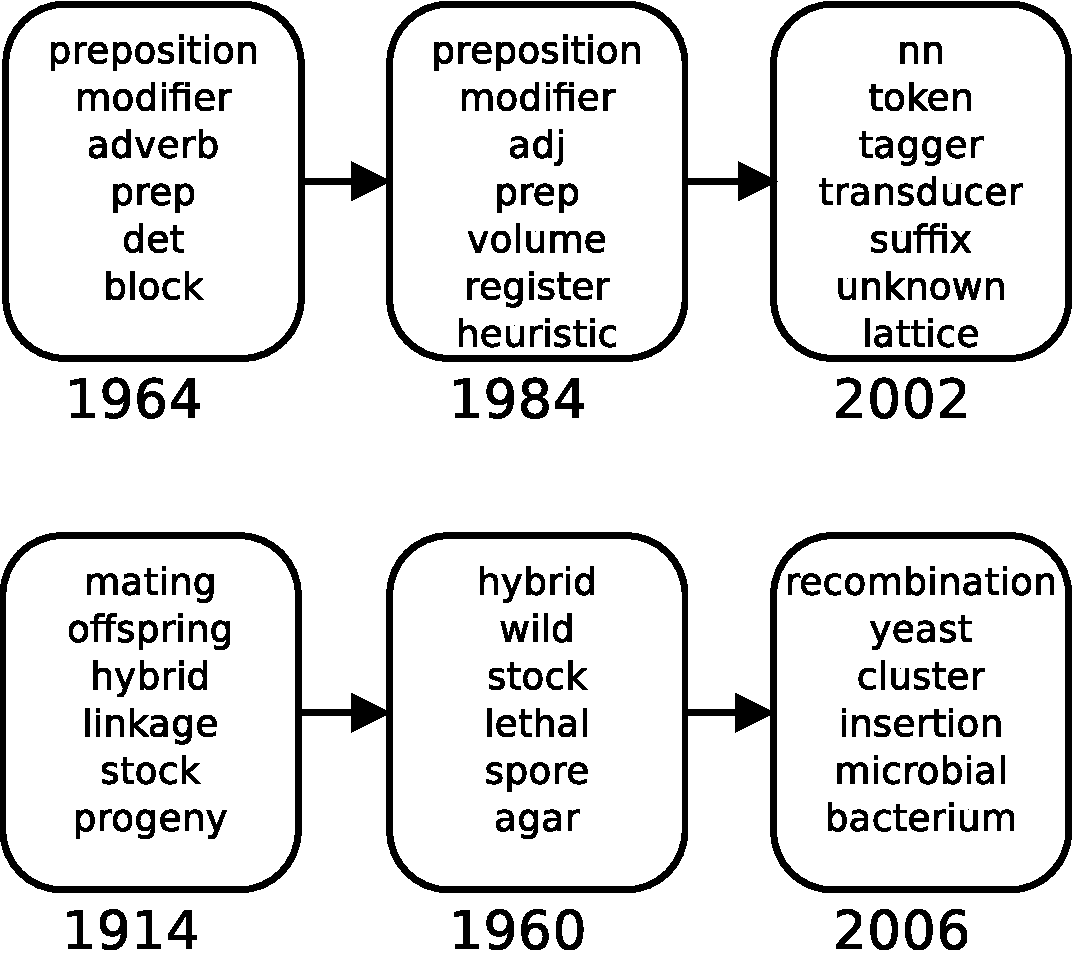
\includegraphics[width=0.7\textwidth]{figs/dynamic_topics.pdf}
  \end{figure}
}

%\frame{
%  \frametitle{A closer look: terms across time}
%  \emph{Genetics of Human Cell Lines, IV. DNA-Mediated Heritable Transformation of a Biochemical Trait}
%  \begin{figure}
%      \begin{centering}
%    \begin{tabular}{cc}
%      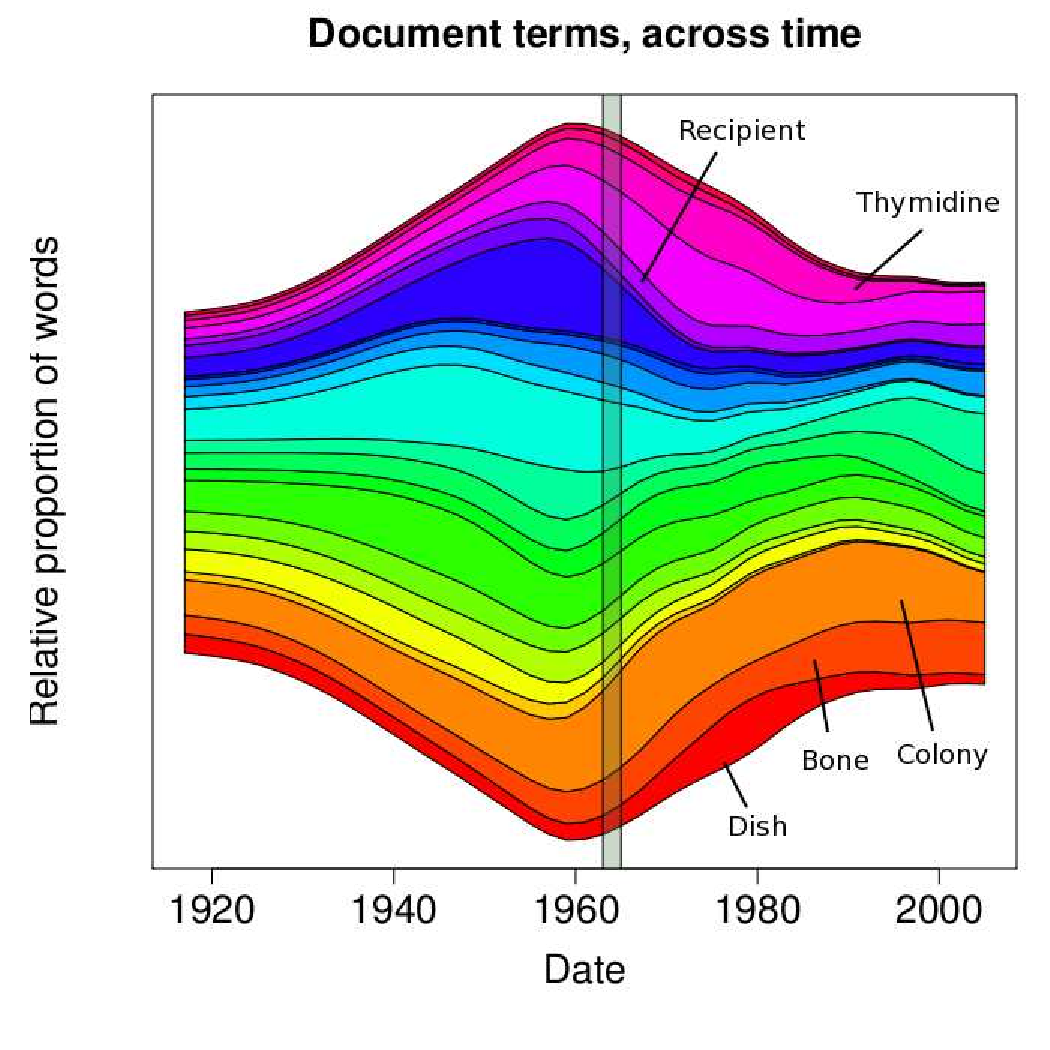
\includegraphics[width=0.45\textwidth]{../figures/genetics_cell_lines_terms_time.pdf}
%      \emph{Genetics of Human Cell Lines}
%    \end{tabular}
%      \end{centering}
%  \end{figure}
%}

\frame{
  \frametitle{A closer look}
  \begin{itemize}
  \item We can inspect documents with high or low scores.
    \begin{itemize}
    \item High influence and high citations
    \item Low influence and high citations
    \item High influence and low citations
    \end{itemize}
  \end{itemize}
}

\frame{
  \frametitle{High influence and high citations}
  \begin{columns}
    \begin{column}[left]{0.3\linewidth}
      \fbox{
	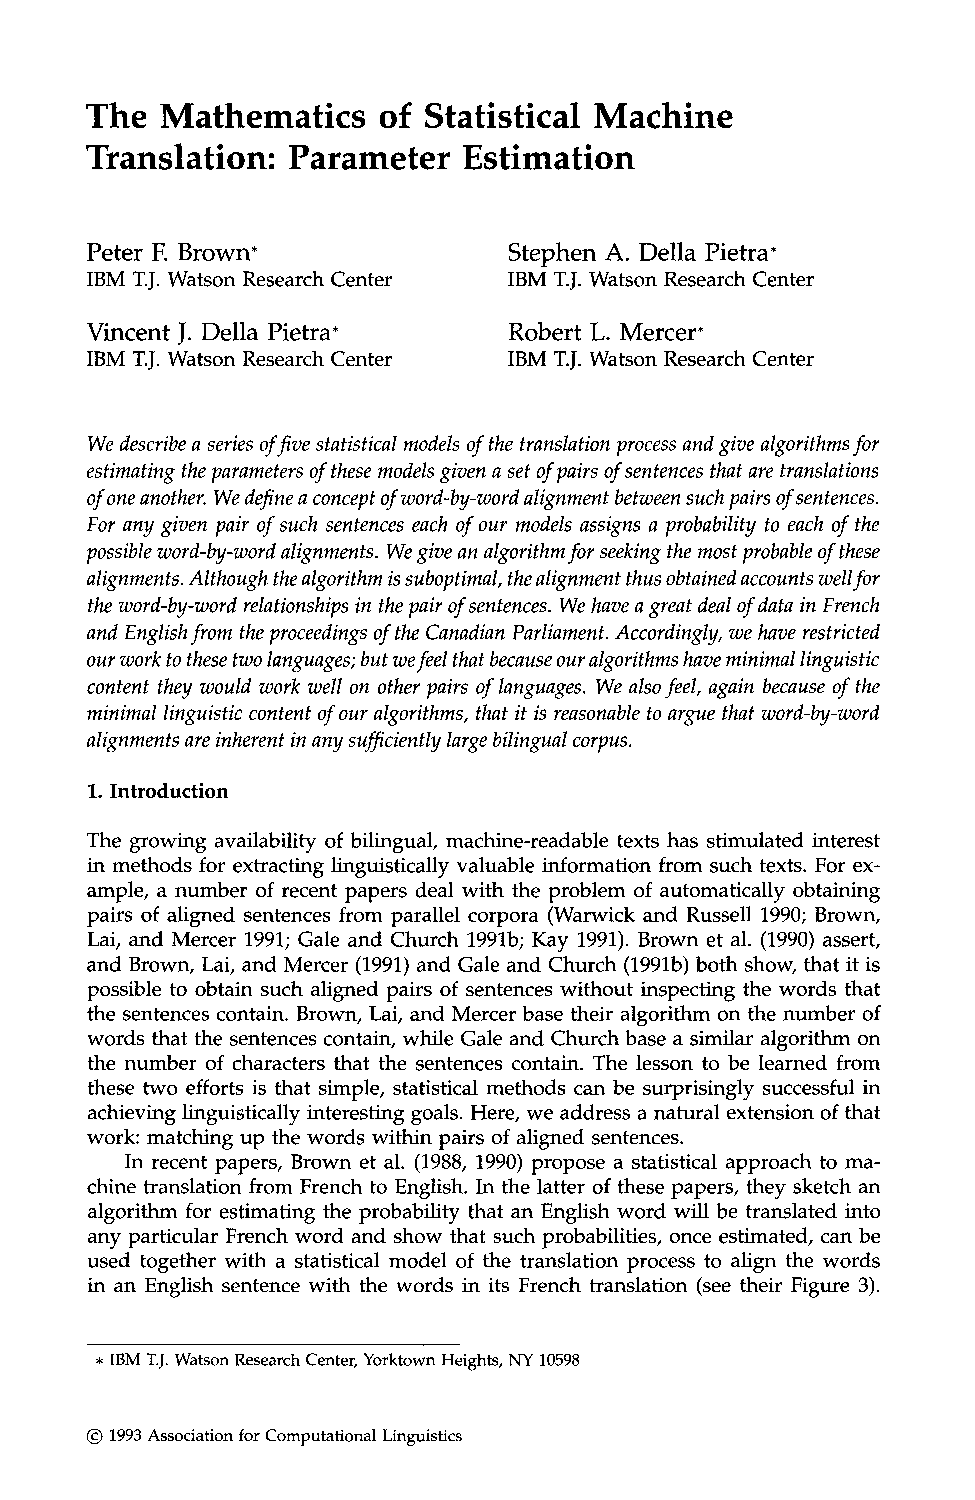
\includegraphics[width=0.9\textwidth]{figs/mathematics_statistical.pdf}
      }
      ACL citations: 7561
      \end{column}
    \begin{column}[left]{0.7\linewidth}
      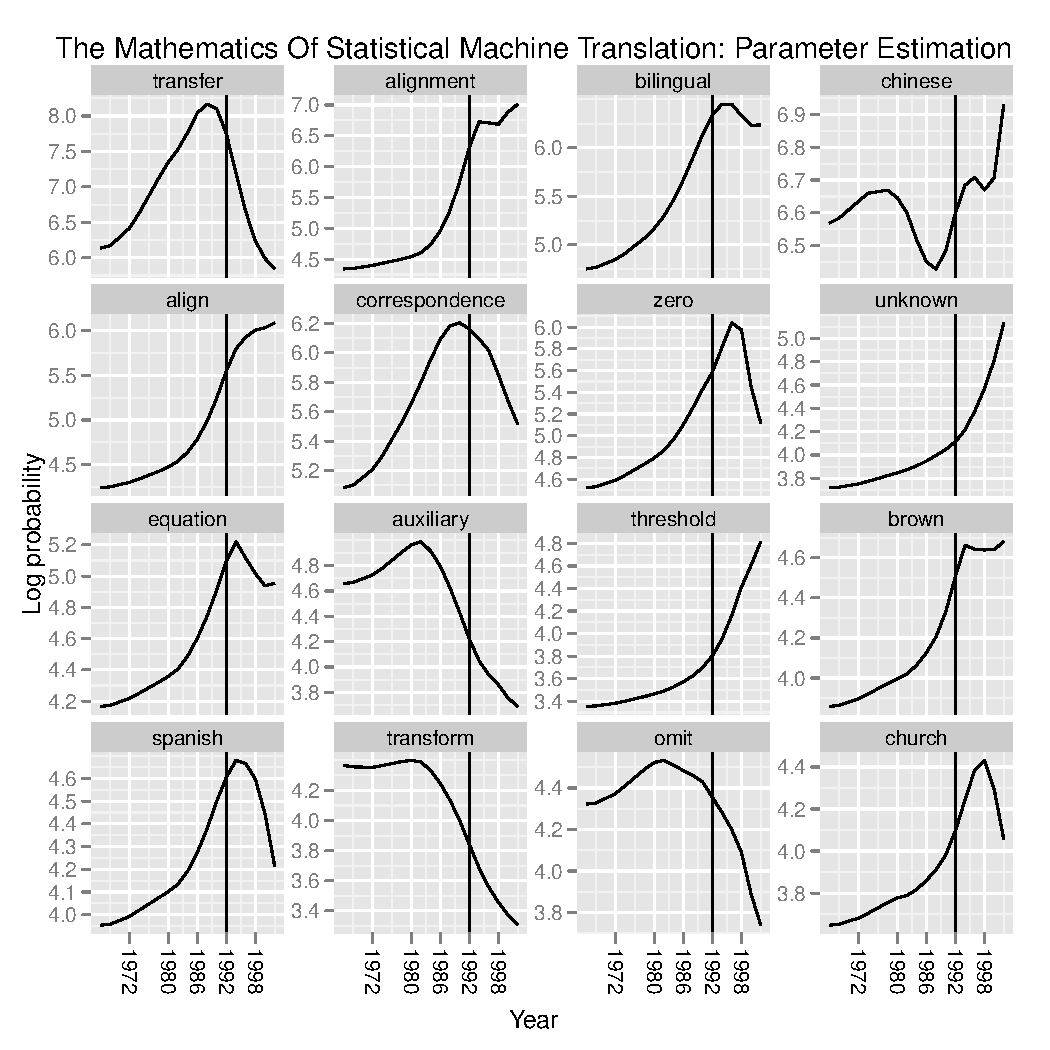
\includegraphics[width=1.0\textwidth]{figs/acl_brown.pdf}
    \end{column}
  \end{columns}

}

\frame{
  \frametitle{Low influence and high citations}
  \begin{columns}
    \begin{column}[left]{0.3\linewidth}
      \fbox{
	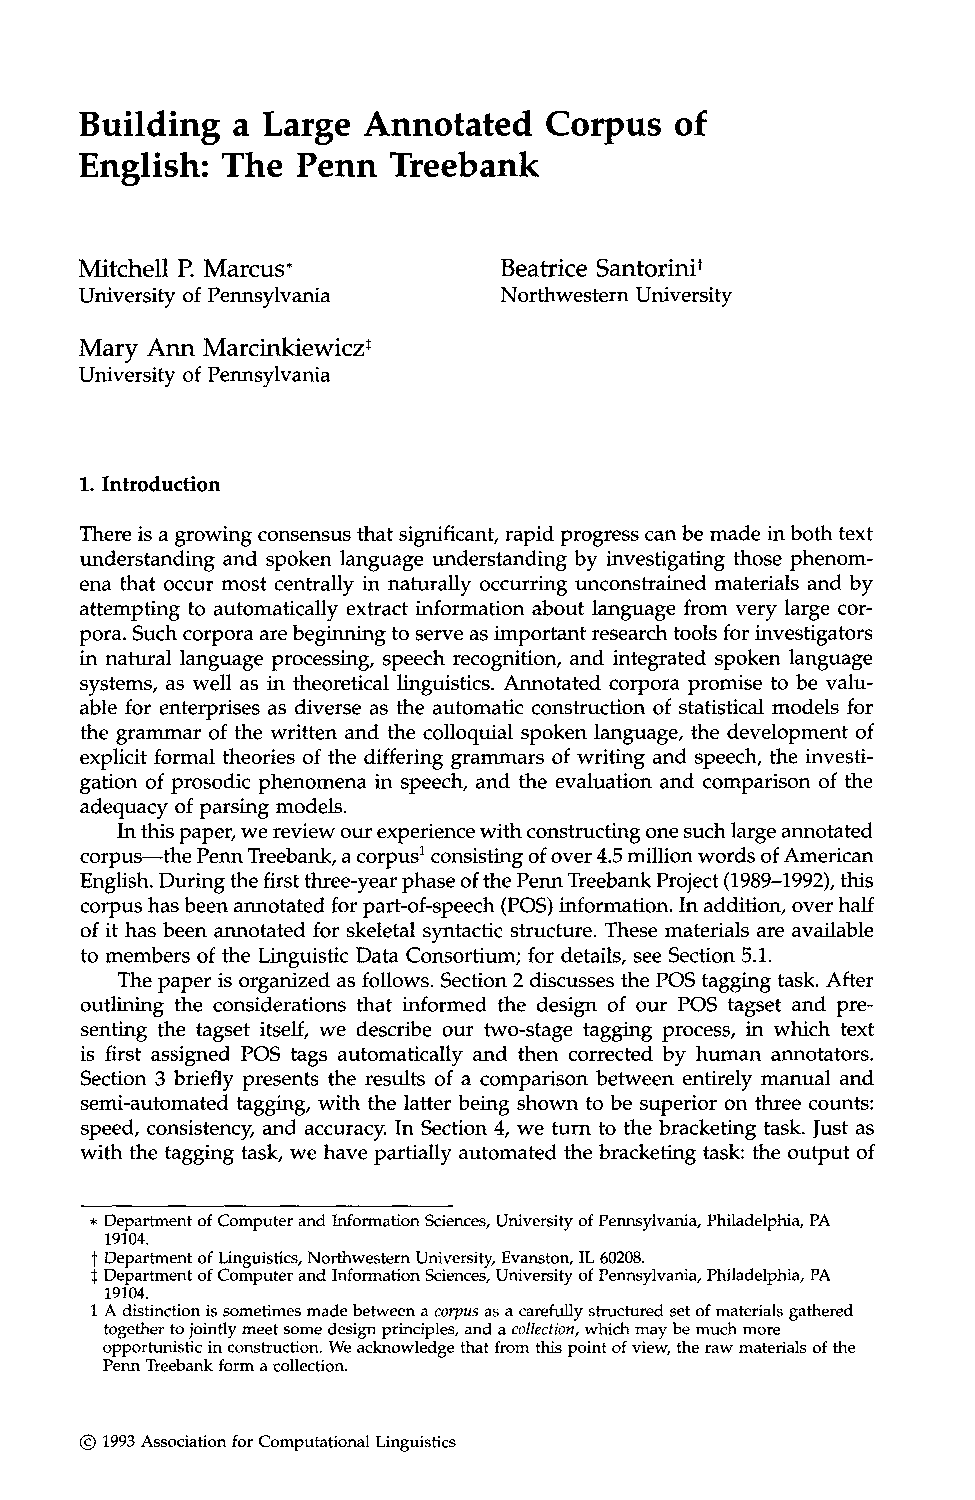
\includegraphics[width=0.9\textwidth]{figs/penn.pdf}
      }
      ACL citations: 2180
    \end{column}
    \begin{column}[left]{0.7\linewidth}
      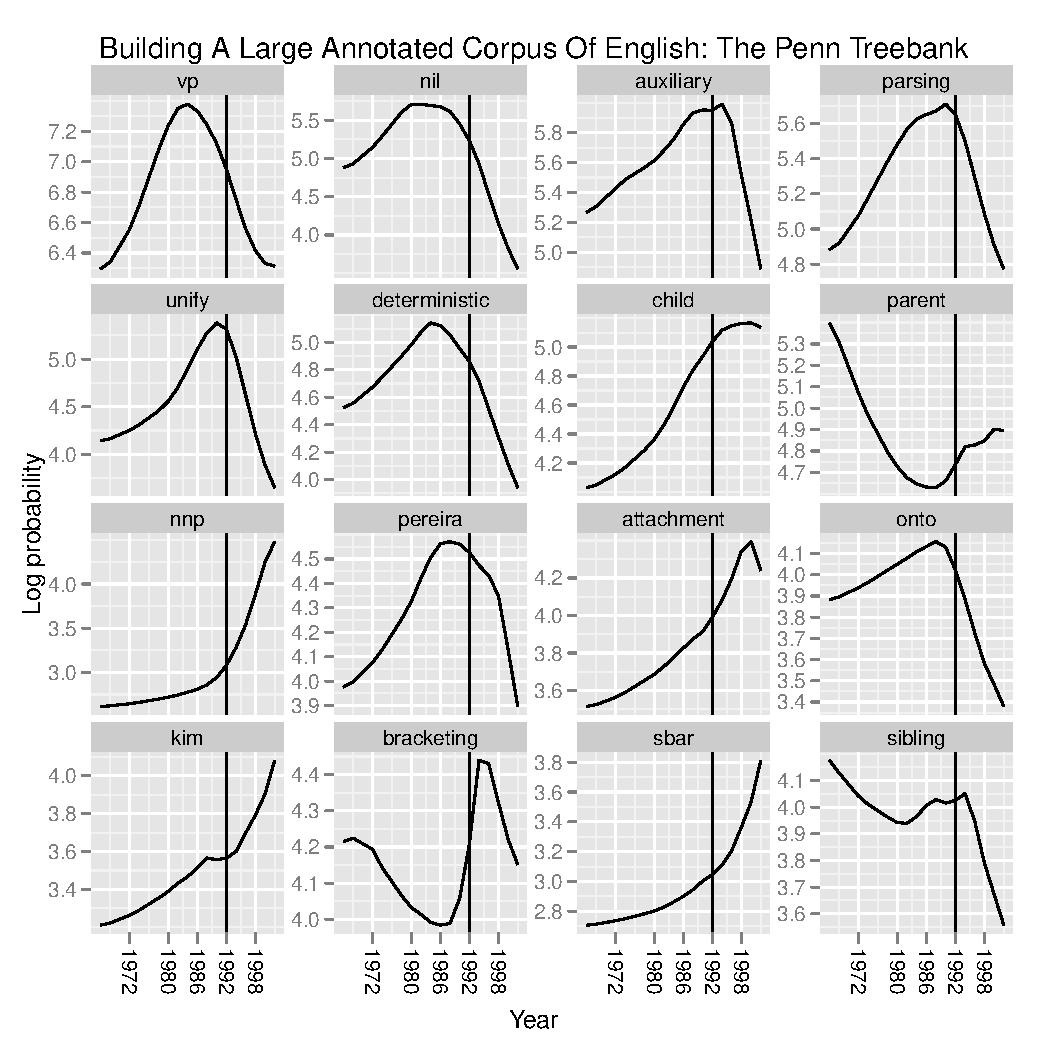
\includegraphics[width=1.0\textwidth]{figs/acl_penn.pdf}
    \end{column}
  \end{columns}
}

\frame{
  \frametitle{High influence and low citations}
  \begin{columns}
    \begin{column}[left]{0.3\linewidth}
      \fbox{
	
\includegraphics[width=0.9\textwidth]{figs/cover_nature.jpg}
      }
      Citations: NA
    \end{column}
    \begin{column}[left]{0.7\linewidth}
      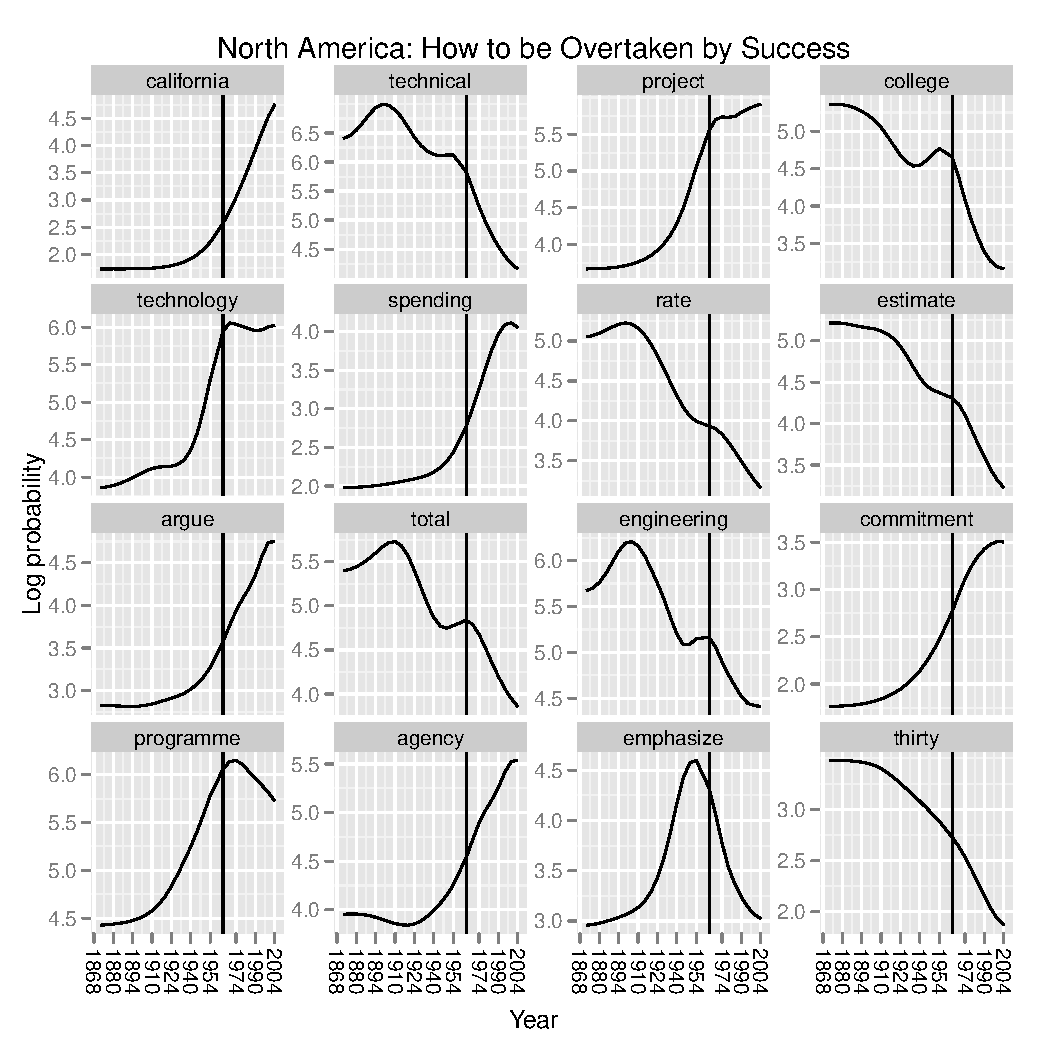
\includegraphics[width=1.0\textwidth]{figs/nature_north_america.pdf}
    \end{column}
  \end{columns}
}

\frame{
  \begin{itemize}
    \item Significant correlation with citations ($p \le 1e-4$)
    \item Window sizes are 4 years for \emph{ACL} and
    \emph{PNAS} and 5 years for \emph{Nature}
    \item Spearman rank correlation 0.37 (ACL); 0.28 (Nature); 0.20 (PNAS)
    \item Also developed a simple baseline which does well:
    0.2 (ACL, PNAS) and 0.26 (Nature)
  \end{itemize}
  \frametitle{Results}
}


\frame{
  \frametitle{Results}
  \begin{itemize}
  \item We can sort articles by decreasing influence and inspect how many citations
    the top $N$ have.
  \item E.g., the top 20\% of \emph{Nature} articles receive 50\% of
    \emph{Nature}'s citations.
  \end{itemize}
  \begin{figure}
    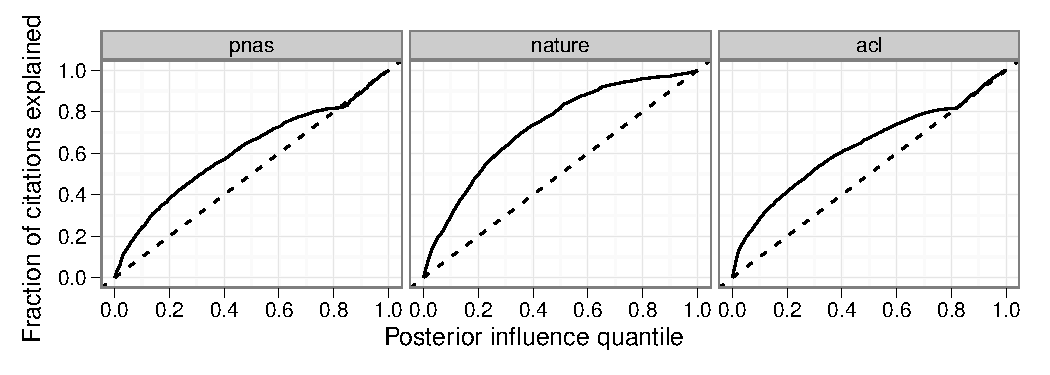
\includegraphics[width=0.8\linewidth]{figs/results_roc.pdf}
  \end{figure}
}

\frame {
  \frametitle{Summary}
  \begin{itemize}
  \item We developed an algorithm that identifies influential documents by analyzing their texts
  \item The Document Influence Model
    \begin{itemize}
    \item Divides the words of a corpus into topics
    \item Infers which articles ``influenced'' their topics
    \end{itemize}
  \item Based only on analyzing the language, our model finds a
    measure of influence that correlates significantly with citation.
    
  \item Some future directions
    \begin{itemize}
    \item Per-document influence envelope \newline
    \item Validation on non-citation data (e.g., usage data) \newline
    \item Application to corpora without citations \newline
    \end{itemize}
  \end{itemize}
}

\frame {
  \frametitle{Contact}
  \begin{itemize}
    \item Sean Gerrish (sgerrish@cs.princeton.edu)
      \newline \url{http://www.cs.princeton.edu/~sgerrish}
    \item David Blei (blei@cs.princeton.edu)
      \newline \url{http://www.cs.princeton.edu/~blei}
  \end{itemize}
  \begin{figure}
    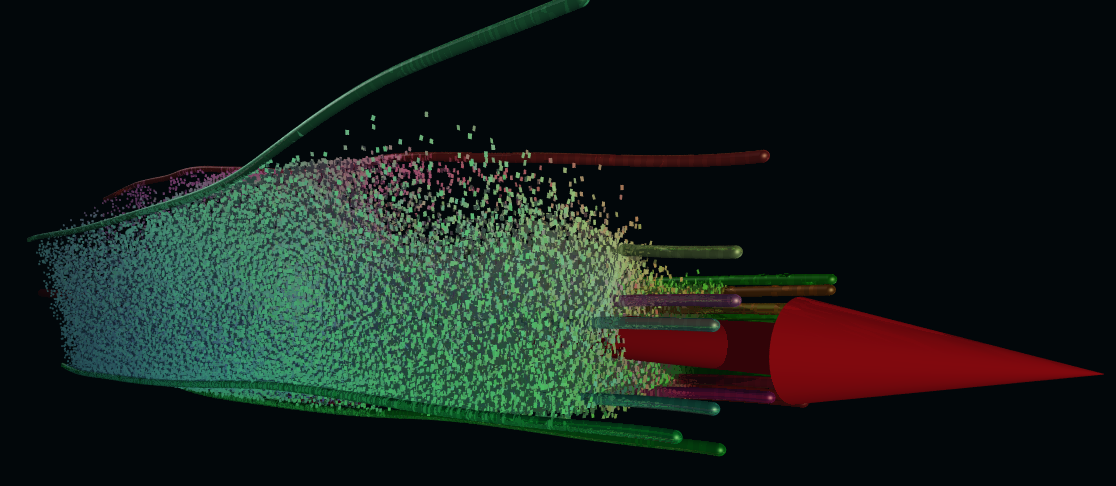
\includegraphics[width=1.0\textwidth]{figs/docs_basic_topics.png}
    \caption{
      \footnotesize
\emph{Nature} articles and their dynamic topics
    \normalsize
}
  \end{figure}
}

\section*{Bibliography and Appendix}

\subsection*{Bibliography}
\begin{frame}[allowframebreaks]
  \frametitle{Bibliography}  \tiny
  \bibliography{../bib} \bibliographystyle{apalike}
\end{frame}

\section{Appendix}

\subsection{Heuristic solution}
\frame{
  \frametitle{Baseline}
  One possible heuristic is simple:
  \begin{itemize}
    \item Define a word's weight at time $t$ as:
      \[
      w_t := \frac{\mbox{Frequency of } w \mbox{ in } [t, t+f] }
      {\mbox{Frequency of }w \mbox{ in [t-b, t]}
      }
      \]
    \item Document $\bm D$'s score is the weighted average of these:
      \[
      \mathcal{I}(\bm D) := \frac{\displaystyle \sum_{w \in \bm D } \mbox{Count}(w) w_t }{ \displaystyle \sum_{w \in \bm D} \mbox{Count}(w) }
     \]
  \end{itemize}
}

\frame {
  \frametitle{Heuristic solution}
  \begin{itemize}
    \item Fast
    \item Easy to implement
    \item Not ``optimal'' in any obvious sense
    \item Does not incorporate information about documents' semantics
    \item Not focused at the level of research contributions
      \begin{itemize}
	\item Too large a hammer
	\item E.g.: cows and health policy around 1986
      \end{itemize}
  \end{itemize}
}

\frame {
  \frametitle{Focus and knowledge contribution}
  The quality of researchers' contributions increases with focus.
\begin{figure}
  \begin{centering}
    \begin{tabular}{cccc}
      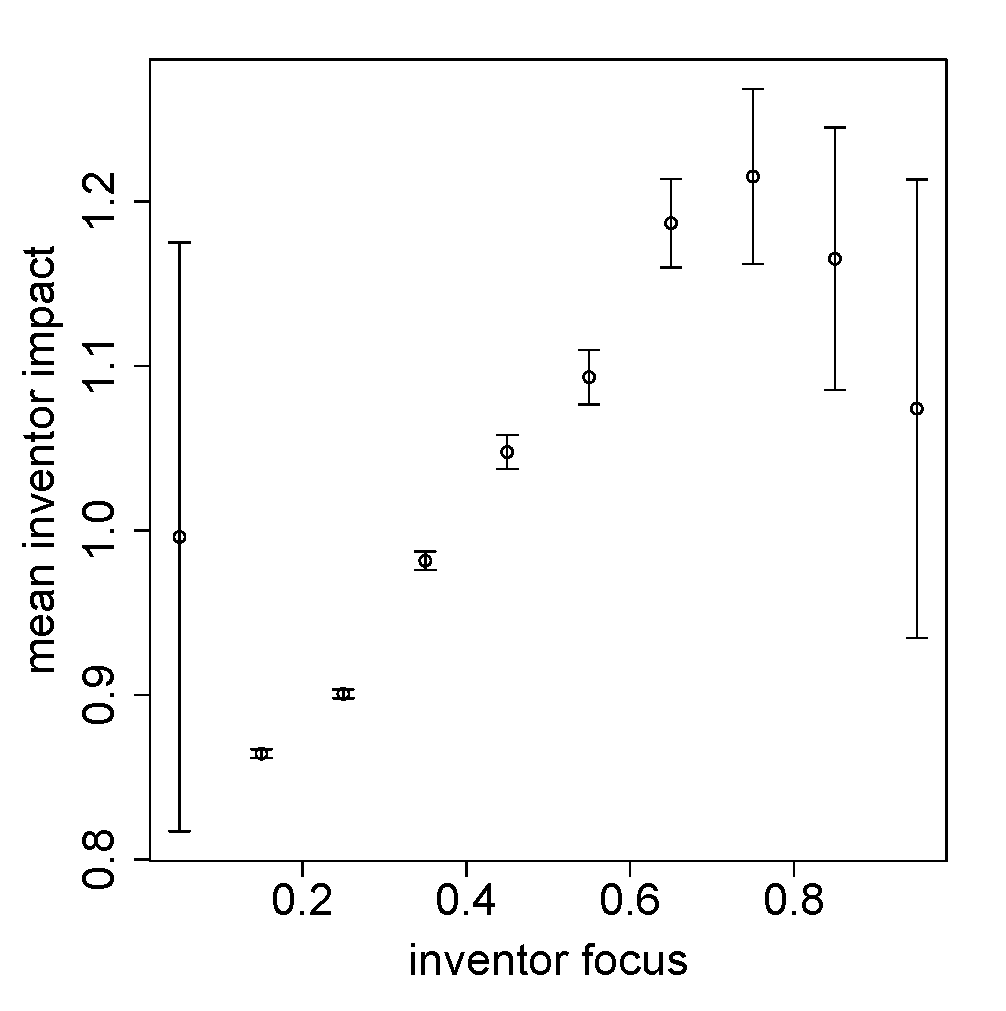
\includegraphics[width=0.27\textwidth]{figs/patentsqvsf.pdf} &
      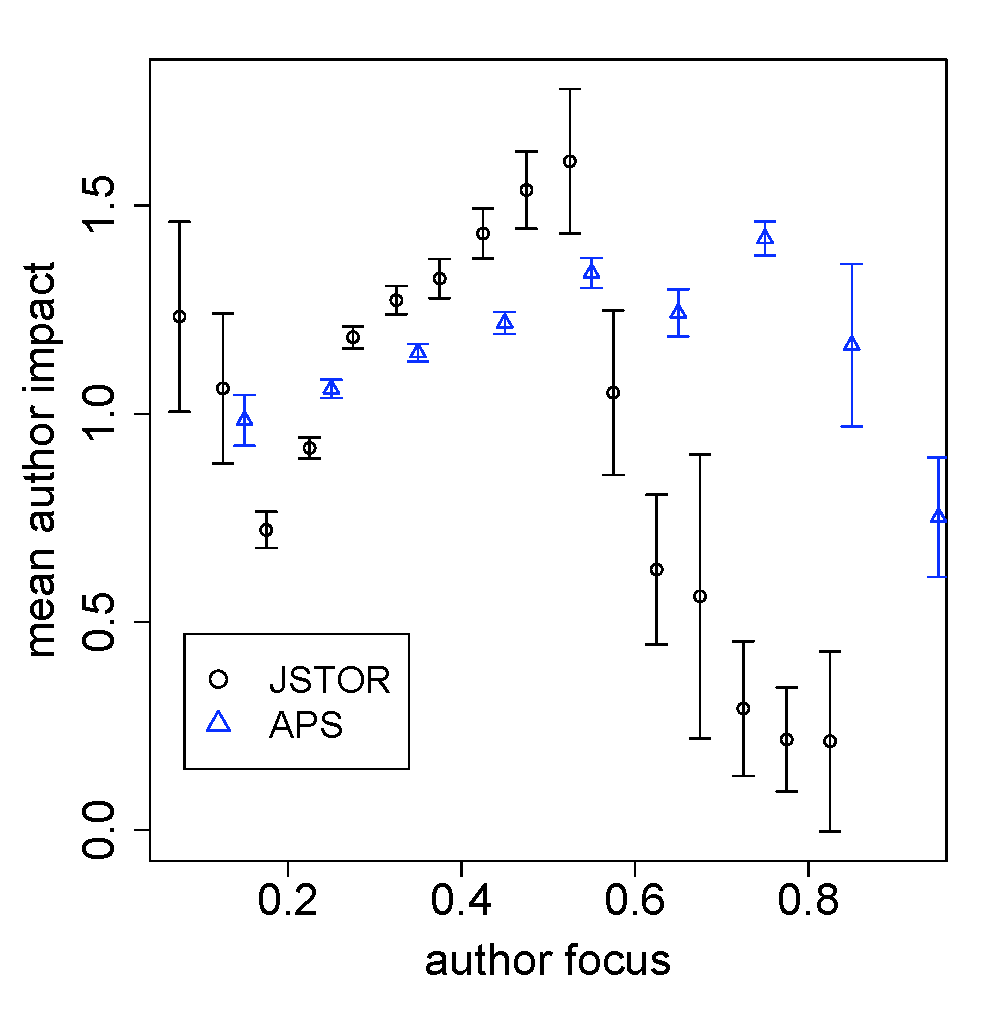
\includegraphics[width=0.27\textwidth]{figs/papersqvsf.pdf} \\
      Patents & Research articles \\
      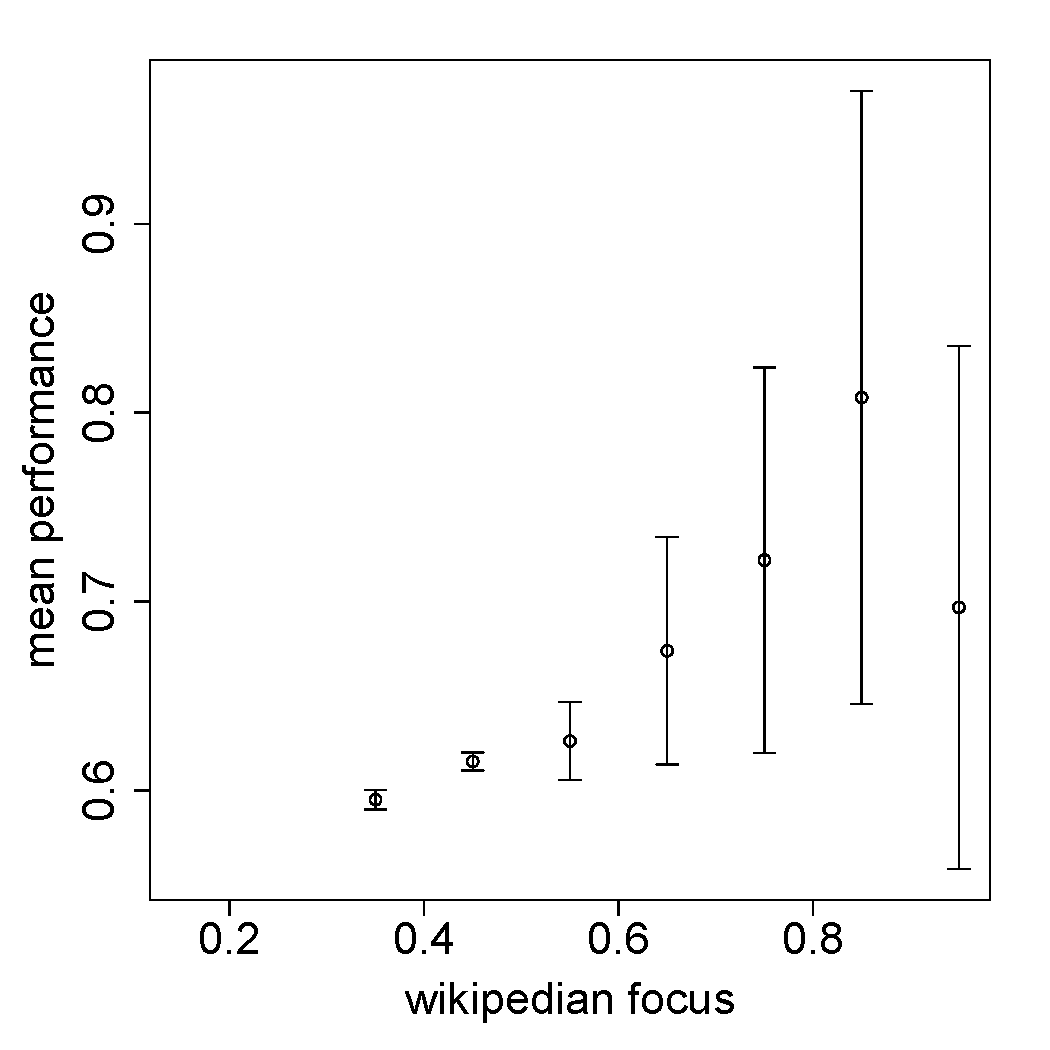
\includegraphics[width=0.27\textwidth]{figs/wikiqvsf.pdf} &
      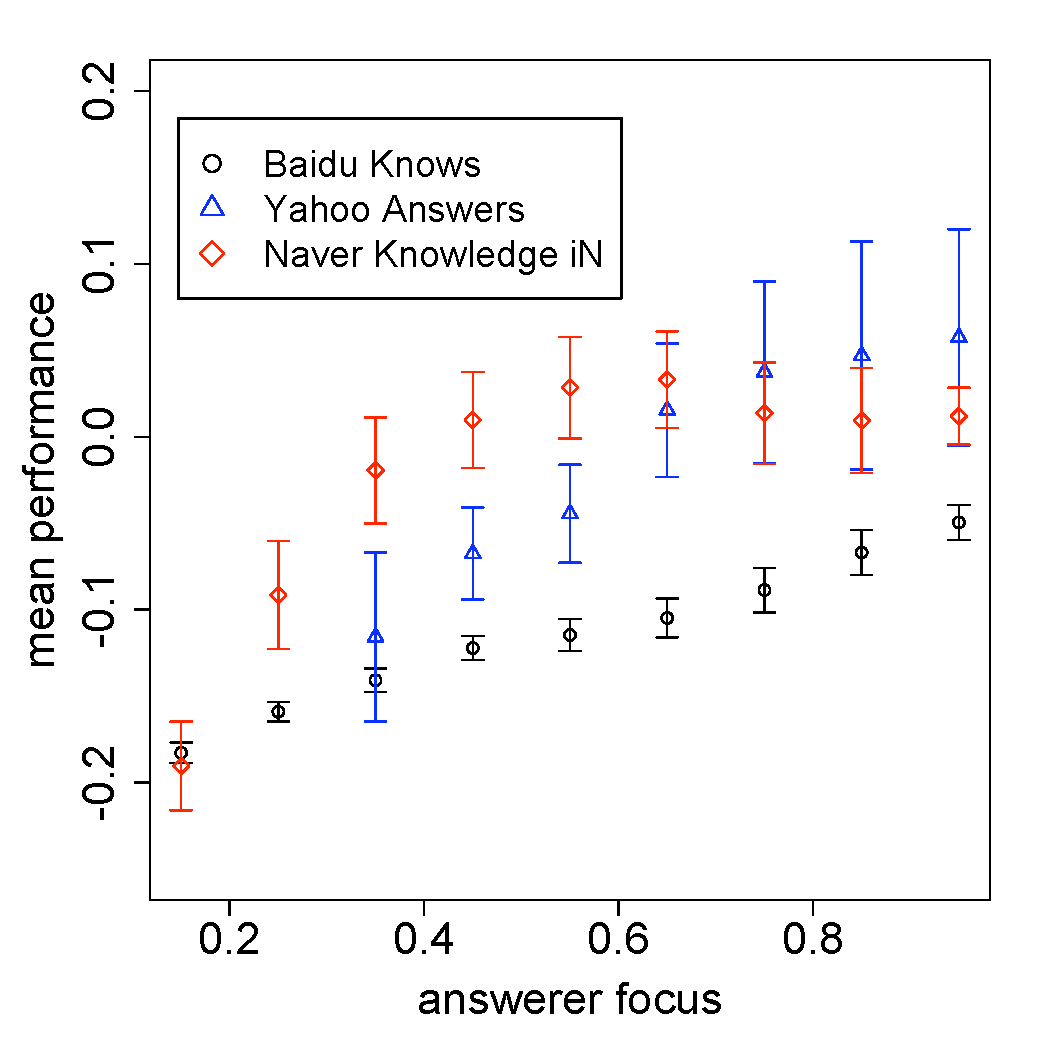
\includegraphics[width=0.27\textwidth]{figs/qnaqvsf.pdf} \\
      Wikipedia & Q\&A forums 
    \end{tabular}
  \end{centering}
  \label{fig:qvsf}
\end{figure}
  \tiny L. A. Adamic, X. Wei, J. Yang, \textbf{S. Gerrish}, K. K. Nam, and
  G. S. Clarkson. \emph{Individual Focus and Knowledge Contribution.}
  Submitted 2010. \normalsize

%  \tiny (Source: Adamic et al., 2010 (under review)) \normalsize
}

\frame {
  \frametitle{Motivation for $\exp(-\beta)$ coefficient in $Infl(t, l, z, w)$}
  \begin{eqnarray}
   & \exp(\beta_t) = \exp(\beta_{t-1}) + Infl_t \nonumber \\
   \iff & 1 = \exp(\beta_{t-1} - \beta_{t}) + \exp(-\beta_t) Infl_t \nonumber \\
   \iff & 1 - \exp(-\beta_t) Infl_t = \exp(\beta_{t-1} - \beta_{t}) \nonumber \\
   \iff & \log(1 - \exp(-\beta_t) Infl_t) = \beta_{t-1} - \beta_t \nonumber \\
   \iff & \beta_t = \beta_{t-1} - \log(1 - \exp(-\beta_t) Infl_t) \nonumber \\
  \end{eqnarray}
  Note that when $\exp(-\beta_t) Infl_t$ is small, we have $\beta_t \approx \beta_{t-1} + \exp(-\beta_t) Infl_t$.
}

\frame {
  \tiny
  \frametitle{Regularized linear regression for $\lv$ updates}
  \begin{eqnarray}
 \label{eq:regression}
g(s, q) := & \Lambda_{\exp(-\mv_{q,k} + \vv_{q,k} / 2)} ( \W_{s,k} \circ \phi_{s,k} ) \\
h(s, q) := & \big( (\W_{s,k} \circ \vphi_{s,k})^T \Lambda_{\exp(-2 \mv_q + 2 \vv_q) + \exp(-2\mv_q + \vv_q)} (\W_{s,k} \circ \vphi_{s,k}) \\
 & + \Lambda_{(\W_{s,k} \circ \W_{s,k} \circ ( \vphi_{s,k} - \vphi_{s,k} \circ \vphi_{s,k}))^T
    (\exp(-2\mv_q + 2\vv_q) + \exp(-2\mv_q + \vv_q)) }
    \big) \\
\lv_{t, k} \gets & 
  \left(
  \frac{\vbv}{\vd} I
  + \left( \sum_{i=t}^{T-1} r(i - t)^2 h(t, i) \right) \right)^{-1} \nonumber \\
  & \left( \sum_{i=t}^{T-1} r(i - t) g(t, i)^T (\mv_{i+1,k} - \mv_{i,k} + \vv_{i,k} - \sum_{j=0 \ldots i, j \neq t} r(i-j) g(j, i) \lv_{j,k} ) \right)
  \nonumber \\
\end{eqnarray}
}

\frame{\frametitle{Dimensionality reduction}
 Bag-of-words model
 \begin{itemize}
   \item Only worry about the word counts in each document
   \item So a document is basically a sparse list of word counts:
  \begin{center}``the cat in the hat'' $\rightarrow$ (0, 0, 1, 0, 2, . . . , 0)\end{center}
 \end{itemize}

 Doing anything with these huge lists is hard
 \begin{itemize}
   \item Popular statistics tools like Principal Component Analysis help us to reduce this to a smaller number
   \item Topic models accomplish a similar thing:
   \begin{center}$10^4$ words $\rightarrow$ 50 topics\end{center}
 \end{itemize}
}

\frame {
  \frametitle{The DIM generative model}
  For time $t = 1, \ldots, T$:
             \begin{itemize}
                \item For topic $k = 1, \ldots, K$: \label{gen:beta} \\
		  Draw natural parameters $\beta_{t,k} | \beta_{t-1,k}, \z_{s<t}, l_{s<t} \sim
		  \mathcal{N}(\beta_{t-1,k} + Infl(t,k), \sigma^2 I)$
               \item For each document $d_t$:
               \begin{itemize}
   	         \item Generate document $d_t$ using traditional LDA with parameters
	          $\alpha_t$ and $\beta_{t}$.
	         \item For topic $k = 1, \ldots, K$,  \label{gen:l}
	           draw document weight $l_{d,k} \sim \mathcal{N}(\textbf{0}, \sigma_d^2 I)$;
               \end{itemize}
             \end{itemize}
}

\frame {
  \frametitle{Topic models - applications} 
  \begin{figure}
    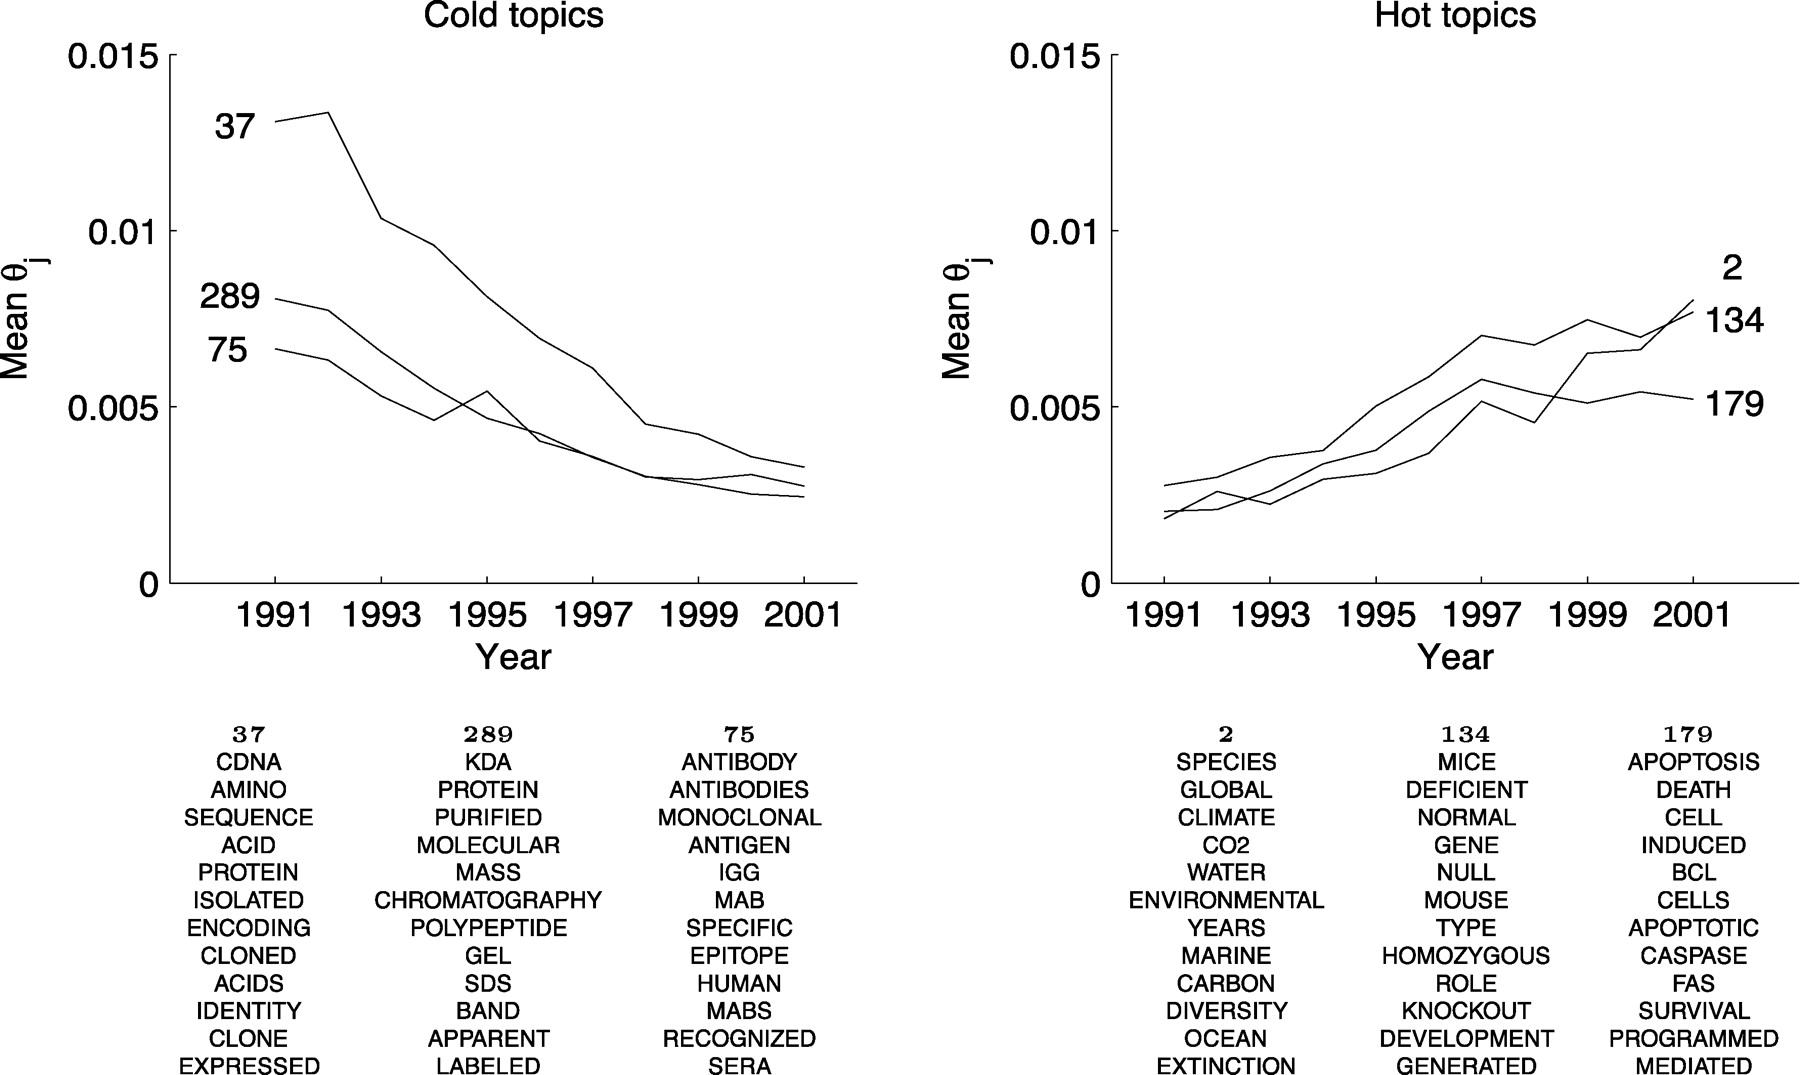
\includegraphics[width=1.0\textwidth]{figs/hot_cold_topics.jpg}
  \end{figure}
  \tiny
  Image source: \cite{griffiths:2004}; Available 2010-01-15 http://www.pnas.org/content/101/suppl.1/5228/F5.large.jpg
  \normalsize
}

\frame {

 \frametitle{Sterling similarity}

 We aimed to use a metric
  that captures three qualities: \emph{variety}, or how many different
  areas an individual contributes to; \emph{balance}, or how evenly
  their efforts are distributed among these areas; and
  \emph{similarity}, or how related those areas
  are.  We use the Stirling measure
  $\mathcal{F}$, which captures all three
  aspects:
\begin{equation}
\mathcal{F} := \sum_{i,j} s_{i j} p_{i} p_{j}, \nonumber
\end{equation}
\noindent where $p_{i}$ is the proportion of the individual's
contributions in category $i$ and $s_{ij}=n_{ij}/n_{j}$ is a measure
of similarity between categories $i$ and $j$, inferred from the number
of joint contributors $n_{ij}$ between two categories $i$ and $j$.

}

\frame{\frametitle{Exploration} Understand the themes in a collection
of documents and how they relate to one another
  \begin{figure}
    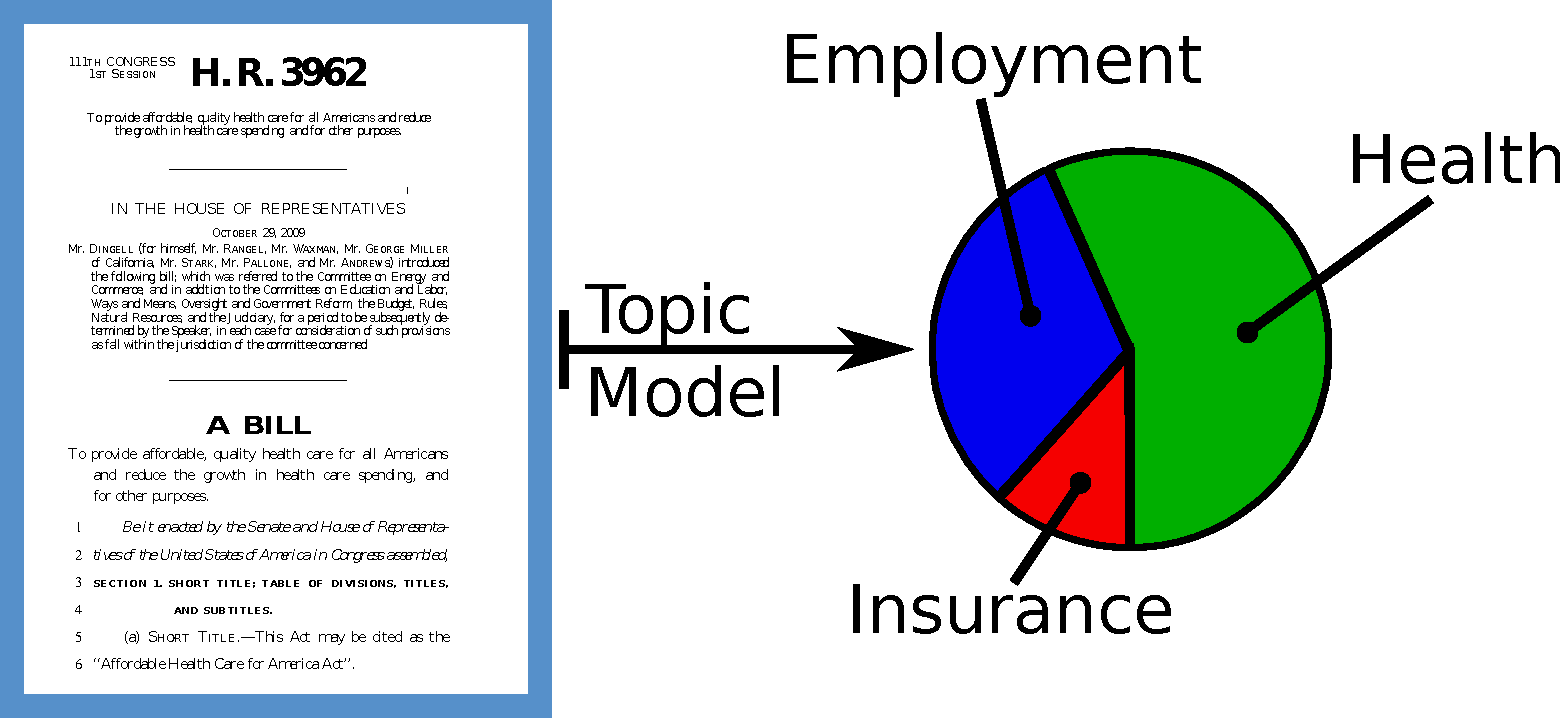
\includegraphics[width=.9\linewidth]{figs/topics.pdf}
  \end{figure}
}

\end{document}
